% ============================================================
%  第五卷 第十四章 二级相变与临界现象（§142–§153）
%  底本：高教社中文版第5版（束仁贵/束莼 译，郑伟谋 校）
%  本章插图 17 幅（图60–图76，多面板图仍为单一 figN.pdf）；
%  习题 6 处（§142、§143、§146、§147、§148、§150，依原书无编号）；
%  正文圈码 83 处（①×44、②×28、③×9、④×2）已全部还原为 \footnote
%  （脚注代理 2026-10-12 转录，页码 p401–p458，逐页对照 pages300 影件；
%   脚注密集页 p409/p426 含 4 注，公式脚注 8 处照原书排入）。
%  遗留照排疑点（见脚注代理报告）：
%   - p426 脚注①"Леванюк А. Л."、"Т. Ⅱ"及 p406 脚注②"ЖЭТФ. 1973"
%     均照原书排（疑为 А. П.、Т. 11、1937 之误排）；
%  已修正的 OCR/原书错误（均对照 原书转换/pages/p-4xx.png 核实）：
%   1. §142 行15279 "液态氮"→"液态氦"（p-403 实为"氦"）；
%      行15293 段末句号补齐（"……子晶格磁矩."）。
%   2. §142 习题 "如 c_0 果 c≠c_0"（OCR 锍断）→"如果 c≠c_0"。
%   3. §143 行15468 "不受溶液中相变所影 α/log"→"所影响"；
%      行15376 T_e→T_c、(143.5) 左端补 η（Φ(P,T,η)，p-391）；行15390
%      "温度 T>T_c③" 圈码复位；行15412 C_y→C_v。
%   4. §144 行15573 "∃′t>0 H′"→"当 t>0 时"（当…时 OCR 乱码，两处）；
%      行15587 "h≫t_t"→"h≫h_t"、"t^γ=0"→"t=0"（OCR 噪声）。
%   5. §145 行15627 式号(145.11)→(145.1)（p-397，指整和式）；
%      行15641 Φ(P,T,η_i^(n)) 后补"）"；行15705 "二极相变"→"二级相变"；
%      行15715 "在相变点附近"重复，删一处（p-401）；
%      行15761 "（k=0 的不可约表示相应于此）"补左括号（p-402）；
%      行15783 φ 函数中 γ→y（cosπ(y∓z) 等，六处，p-404）；
%      行15797 "(4)^4+4^4"→(φ_1^4+φ_2^4)（p-404）；
%      行15803 8C 坐标表中重复的 (3/4 3/4 3/4)→(1/4 3/4 3/4)（p-404）；
%      行15853 "dot∓是问题中"→"于是问题中"（p-406）。
%   6. §146 行15863 ΔΦ_t②（OCR 𝒬→②，p-406）；行15887 "增长Φ."→"增长①."
%      （p-407）；行15899 b=B/V^α→b=B/V（p-407）；行15927 R_oin→R_min；
%      行15961 增大J→增大①；行16016 人名按 p-410 复原：
%      (А. П. Леванюк, 1959; В. Л. Гинзбург（金兹堡）, 1960)；
%      行16131 A.II.eBHk→(А. П. Леванюк, 1963)（p-414）。
%   7. §147 行16062 e^{μNτ}→e^{μN/T}、E_n→E_N、dT_N→dΓ_N（Γ 被 OCR 作 T，
%      (147.1)(147.2) 及全文；p-411/412）；行16090 Ω[η~] 展开式按 p-412 复原；
%      行16107 "η=η~ 附近"补排；行16111 "依赖干截断参数"→"依赖于截断参量"；
%      行16125 "按所有可能 η_k 方式配对"→"按所有可能方式配对"（p-413）；
%      习题 (1) 中 g^{k^2}→gk^2、V_0^{k_0}→V∫_0^{k_0}（p-414）、
%      C_ν−C_{p0}→C_p−C_{p0}（p-414）。(147.5) 指数分母及习题、(147.7) 后
%      高斯分布中的 T_c 系原书排印如此（p-412/413），照排。
%   8. §148 (148.1) 按 p-415 复原为 C_p=T_c(dP_c/dT)(∂V/∂T)_P（当 T→T_c 时）；
%      (148.5) η_sp/η_ind 按词头复原（行16257/16260）；(148.6) |t|^...→|t|^{−ν}；
%      (148.8) χ∝|t|·γ→|t|^{−γ}；行16227 h_·/h_↑→h_t（三处）；
%      行16269 |t|^{2…α−β}→|t|^{2−α−β}；(148.14) 后 h/t^{βδ}（行16353）；
%      (148.19) 按 p-418 复原为 f(x)=常数（当 x→0 时）；
%      (148.20) 按 p-418 复原两极限；行16306 ⟨(Δη)²⟩_ν→⟨(Δη)²⟩_V；
%      (149.6)(149.7) 中 h^{μν}→h^{μ/ν}、h^{#}→h^{μd}（p-420/421）；
%      (149.9)(149.10) 分母 t^{2νμ}→t^{2ν/μ}、(−1)^{νd}→(−t)^{νd}（p-422）；
%      (149.11) "=5"→"=ζ"（p-422）；行16514 G(r) 式按 p-422 复原；
%      行16391 行首"标度不变性假设(L. Kadanoff, 1966; А. З. Паташинский,
%      В. Л. Покровский, 1966)"人名按 p-420 复原。
%   9. §150 (150.10) T_c²a_c²→T_c a_c²（按 p-425 及上下文"两倍"关系，
%      原书该处 T 上衍上标 2，属排印错误）；行16648 "项四次作为系数"→
%      "四次项作为系数"；习题按 p-427 复原：Φ_t（OCR Φ_∥）、
%      "（dη/dx）²项的系数变为零…考虑（d²η/dx²）²阶次的项"（原书两项
%      互换，物理上栗弗席兹点为 g=0，已按(1)式与 g(P_L,T_L)=0 更正）；
%      习题势值 Φ_Ⅲ=Φ_0−(1/3)(ò/B) 按 ½Ãη_0²+(3/8)Bη_0⁴ 取极小应为
%      −(1/6)(ò/B)，相应一级相变线方程原书 A=g²/[f(√6−2)] 按推导应为
%      A=g²/[(√6+2)f]，均已更正（原书两处排印错误，p-427）。
%  10. §151 (151.5) Σ_r 带撇（r 偶）照 p-429 排；(151.6) 前二式 ∑_{r=0}、
%      (151.8) ∑_{r=1} 依原书；行16851 方向图按 p-431 复原（1右2上3左4下）；
%      行16854 "最后一步不应该沿箭头ν所指的方向"按 (151.9) 及 p-432
%      "不可从右面"更正为"不应该与箭头ν所指的方向相反"（译文脱"相反"）；
%      行16874 系数矩阵 A→Λ（p-432）；行16776 多项式项按 p-429 复原
%      （含 c) 项 σ³_{k−1,l−3}，原书如此）；(151.14) "bT_c bln"→"bT_c ln"；
%      (151.15) "常数·"按 p-434 复原。
%  11. §152 行17031 8V³→δV³、8F→δF（δ 被 OCR 作 8）；行17049
%      "∃≤ι=0 H}"→"当 t=0 时"；行17103 补句读；行17112 p_t→p=bt；
%      行17159 (2/n_c) 前按 p-438 复原 φ(k) 式。
%  12. §153 (153.4) (−l)^β→(−t)^β；(153.6) |η|^∘→|η|^δ；
%      (153.10) 按 p-441 复原为 p−bt∝t^γ[c_1η+c_3η³t^{−2β}+⋯]
%      （当 t≫|η|^{1/β} 时）；(153.11) 按 p-442 照排 |h|^{2−α}；
%      行17248 "p_1 和t"→"p 和t"（p-441）；行17318 (B.Ⅱ.,1972)→
%      (В. Л. Покровский, 1972)（p-442）；行17333 V_7→Vη、
%      "常数·"按 p-443 复原；行17336 引用(153.14)→(153.4)（所引为
%      共存曲线密度规律，原书排印误）；行17342 η_t+η_2→η_1+η_2。
%  13. 习题内部编号公式（§142(1)(2)、§147(1)(2)、§150(1)(2)）原书以
%      (1)(2) 编号并在题解中引用，用 \tag 排（自动编号无法给出节内(1)）。
%  遗留问题：
%   - 行15901 "Ω_t(T,μ)" 与行15891 "Ω_r(T,μ)"：OCR 两读，按 p-407 脚注
%     体例（角标 t=整个物体）取 Ω_t(T,μ)。
%   - 行15935 "然后，下步处理类似于§116"之"下步"，p-408 影件难以确认是否
%     为"下一步"，照 OCR 排。
%   - 行16027 "这个定理成立的温度范围"，p-410 影件似为"定理"，照排。
%   - §145 行15753 χ_{kα,kβ}（OCR ββ），p-402 影件小字难辨，按上下文取 kβ。
%   - §147 (147.5) 指数中 T_c、习题中 T_c：与(147.1) 的 T 不一致，原书如
%     此（俄文版亦然），照排未改。
%   - §150 习题"（A. Michelson, 1977）"人名原书如此，照排。
% ============================================================
\chapter{二级相变与临界现象}

\section{二级相变}

在§83中曾经指出：具有不同对称的两相（晶态和液态、不同型的晶态）之间，不能像液态和气态之间所可能的那样以连续的方式发生相变.在每一种状态下，物体具有这种或者另一种对称，因此总是可以说出它属于两相中的哪一相.

不同型晶态之间的转变通常通过相变实现，相变中晶格突然重构，而物体的状态经历跃变.但是除了这种跃变以外，还可能有另外一类与对称的改变有关的相变.为了阐明这种相变的性质，我们举一个具体例子.在高温下，BaTiO$_3$具有立方晶格，其晶胞如图60所示（Ba原子在顶点，O原子在面心，Ti原子在胞的体心）.当温度降到某一确定值时，Ti原子和O原子开始沿着立方体某一条棱的方向相对于Ba原子移动.显然，只要这种位移一开始发生，晶格的对称就立刻改变：从立方对称变到四方对称.

\par\nopagebreak\noindent\begin{minipage}{\linewidth}\centering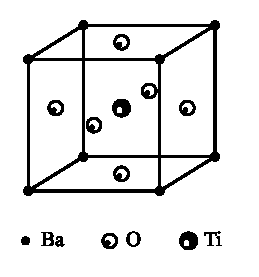
\includegraphics[width=5cm]{fig60.pdf}\\[0.3em]{\small 图 60}\end{minipage}\par\nopagebreak

这个例子的特征在于：物体的状态并不发生任何跃变.晶格中原子的位形\footnote{为了简化讨论起见，我们约定谈及原子的位形及其对称时，视原子如同静止.实际上，应该讲原子在空间不同位置的概率分布和这种分布的对称.}以连续的方式变化.但是，原子偏离它们原始对称位形的位移不管多么小，都足以使晶格对称立刻改变.以这种方式实现的从一种晶型到另一种晶型的转变，称为二级相变，以区别于通常的相变，相应地后者称为一级相变\footnote{二级相变点也称为居里点（特别是与物体的磁结构变化有关的相变点）.}.

因此，说二级相变是连续的，指物体的状态以连续的方式变化.然而应当强调，在相变点对称的变化自然是跳跃的，而在每一时刻可以说出物体属于两相的哪一相.但是，在一级相变点，两种不同状态的物体处于平衡，而在二级相变点两相的状态等同.

除了物体对称的改变由原子位移引起（如以上所举的例子）的情形以外，在二级相变过程中对称的改变也可由晶体排序上的变化而引起.在§64中已经指出，如果某种给定类型的原子所可能占有的格点数目超过该种原子本身的数目，那么出现排序的概念.我们把该种原子在完全规则晶体中所处的位点称为“本座”，相应地，当晶体“无序化”时这种原子的一部分所转移到的位点称为“异座”.在我们感兴趣的许多二级相变问题中，“本座”和“异座”在几何上是完全相似的，其区别只在于该种原子处于这两种格点上的概率不同\footnote{应当注意，这里总可以认为：原子处于“本座”的概率大于处于“异座”的概率，只不过因为否则就应当颠倒叫法.}.现在如果在本、异座的概率相等（当然它们不会等于1），那么所有这些格点都变成等效的，因而出现新的对称元素，也就是说晶格对称性提高.这样的晶体称为无序晶体.

我们就以上所述举例说明.完全有序的CuZn合金具有立方晶格，其Zn原子譬如说位于立方胞的顶点，Cu原子位于体心（图61a；简立方布拉维格子）.当温度升高而发生“无序化”时，Cu原子和Zn原子改变位置，这就是说，两种原子在所有格点上出现的概率都不等于零.只要Cu（或Zn）原子处于胞顶点和体心的概率不一样（晶体不完全无序），那么这些格点仍旧不是等效的，而晶格仍旧保持原来的对称.但是这些概率一旦相等，所有的格点就变成等效的，因而晶体的对称提高，出现新的平移周期（从胞顶点到体心），因而晶体具有体心立方的布拉维格子（图61b）\footnote{原则上可能发生如下情况：有序化的出现并不引起晶体对称的改变.在这种情形下二级相变是不可能的：即使有序晶体会以连续方式过渡到无序，比热也不会发生任何跃变（见后）.当然，在这种情形下一级相变是可能的.}.

\par\nopagebreak\noindent\begin{minipage}{\linewidth}\centering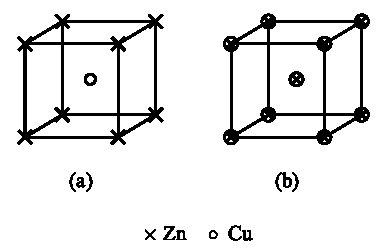
\includegraphics[width=6.5cm]{fig61.pdf}\\[0.3em]{\small 图 61}\end{minipage}\par\nopagebreak

以上我们只讨论了不同晶型之间的转变.但是二级相变未必就应该涉及晶格中原子位形的对称变化.以不同的别种对称性质描述的两相之间，也可通过二级相变实现相互转变.铁磁或反铁磁物质居里点就是例子；在这种情况下，我们考虑物体中基本磁矩排列对称的改变（更确切地说，物体中电流 $j$ 的消失，参看§128第一个脚注）.金属转变为超导状态（没有磁场时）和液态氦转变为超流态也都是二级相变.在这两种情形下，物体的状态都以连续的方式变化，但是在相变点，物体都获得全新的性质.

因为在二级相变点两相的状态完全一致，显然，正好在相变点时物体的对称总应该包含两相的全部对称元素.以后将证明：相变点处的对称与该点一侧的对称即两相中一相的对称处处一致.因此，在二级相变时物体对称的改变具有如下非常重要的共同性质：两相中的对称彼此联系，一相对称较高，而另一相较低\footnote{必须提醒，这里所说的高对称应包含另一较低对称的所有元素（转动、反映、平移周期），以及此外的附加元素.上述要求是二级相变可能发生的必要条件，但绝非充分；下面将看到，在这种相变下对称的可能变化还服从进一步的限制.}.必须着重指出：在一级相变时，物体对称的改变不受任何限制，两相的对称可以彼此毫无共同之处.

在绝大多数已知的二级相变情形下，对称较高的相，对应于较高的温度，而对称较低者对应于低温度.特别是，从有序态到无序态的二级相变总是在温度升高时发生.然而，该规则不是热力学的规律，因此容许有例外\footnote{罗谢尔盐的低居里点便是一例，在该点以下晶体属于斜方晶系，而该点以上属单斜晶系.}.

为简便起见，以下约定把更对称的相称为对称的，而把欠对称的相称为非对称的.

为了定量地表征物体在经过相变点时结构的变化，可引入所谓的序参量 $\eta$，它的定义方式应使得它在非对称相中取非零值（正或负），而在对称相中等于零.因而，对于与原子偏离其对称相中位置有关的相变，$\eta$ 可理解为该偏移量.对于和晶体排序改变有关的相变（如上述的CuZn合金例），参数 $\eta$ 可以定义为
\begin{equation*}
  \eta=\frac{w_{\mathrm{Cu}}-w_{\mathrm{Zn}}}{w_{\mathrm{Cu}}+w_{\mathrm{Zn}}},
\end{equation*}
式中 $w_{\mathrm{Cu}}$ 和 $w_{\mathrm{Zn}}$ 分别为Cu和Zn原子处于任一给定格点的概率.对于磁相变，$\eta$ 可取作铁磁体的单位体积宏观磁矩或者反铁磁体的子晶格磁矩.

我们再次强调：物体对称的改变（增加）只发生在 $\eta$ 精确地变成零的时刻；只要序参量不等于零，不管多小都导致对称降低.在过二级相变点时，$\eta$ 连续地变为零，没有突变.

在二级相变点不存在状态的跃变，这就使得物体状态的热力学函数（熵、能量、体积等）在过相变点时保持连续.因此，二级相变不同于一级相变，不伴有放热或吸热.但是下面将要看到：上述这些热力学量的导数（即比热、热膨胀系数、压缩率等）在二级相变点处有跃变.

值得注意：从数学上看，二级相变点是热力学量特别是热力学势 $\Phi$ 的某种奇点（这种奇点的特性将在§148，§149讨论）.为阐明这一点，首先提醒一级相变点并不是奇点，它只是两相热力学势 $\Phi_1(P,T)$ 和 $\Phi_2(P,T)$ 彼此相等的点，并且相变点两侧的函数 $\Phi_1$ 和 $\Phi_2$ 中的每一个对应于物体的某一平衡态（虽然可能是亚稳的）.然而，在二级相变中，如果形式地从相变点的另一侧看任一相的热力学势，那么它根本不对应于任何平衡态，也就是说，不对应于 $\Phi$ 的任何极小值（在下一节中我们将看到：对称相的热力学势在相变点的另一侧甚至会对应于 $\Phi$ 的极大值）.

根据以上所述，在二级相变中不可能有过热或过冷的现象（它们可以出现在通常的相变中）.在这种情况下，两相中的任一相都不可能越过相变点而在另一侧存在（当然，这里没有考虑建立原子平衡分布所需要的时间，它在固态晶体中可以很长）.

\begin{xiti}

设 $c$ 是二元固溶体一种成分的原子浓度，而 $c_0$ 是该原子“本座”的浓度.如果 $c\neq c_0$，晶体不可能完全有序.假定差 $c-c_0$ 很小而且晶体几乎是完全有序的，确定原子在“异座”的浓度 $\lambda$，并将之用 $c=c_0$ 时 $\lambda$ 该有的值 $\lambda_0$（对于给定的P和T）来表示（C.~Wagner，W.~Schottky，1930）.

解：我们总是只考虑一种成分的原子，引入原子在异座的浓度 $\lambda$ 及本座不为该原子占有的浓度 $\lambda'$；浓度相对于晶体中全部原子总数而定义.显然，
\begin{equation}
  c-c_0=\lambda-\lambda'.\tag{1}
\end{equation}
把整个晶体看成是“溶液”，“溶质”为处于异座的原子与不为原子占有的本座，而处于本座的粒子起溶剂的作用.于是，原子从异座过渡到本座，可以看成是溶质（具有小浓度 $\lambda$ 和 $\lambda'$）之间发生“化学反应”生成溶剂（浓度$\approx$1）.对这种“反应”运用质量作用定律，我们得到 $\lambda\lambda'=K$，此处K仅与P和T有关.在 $c=c_0$ 时应该有 $\lambda=\lambda'\equiv\lambda_0$，所以 $K=\lambda_0^2$，结果
\begin{equation}
  \lambda\lambda'=\lambda_0^2.\tag{2}
\end{equation}
从(1)和(2)可得所求的浓度
\begin{equation*}
  \lambda=\frac{1}{2}\Bigl[(c-c_0)+\sqrt{(c-c_0)^2+4\lambda_0^2}\Bigr],
\end{equation*}
\begin{equation*}
  \lambda'=\frac{1}{2}\Bigl[-(c-c_0)+\sqrt{(c-c_0)^2+4\lambda_0^2}\Bigr].
\end{equation*}

\end{xiti}

\section{比热的跃变}

二级相变定量理论的出发点，在于考虑在相对于对称态有一定的偏离时（即在给定的序参量 $\eta$ 下）物体的热力学量；例如，把物体的热力学势表示为 $P$，$T$ 和 $\eta$ 的函数.当然，这里必须注意，在函数 $\Phi(P,T,\eta)$ 中，变量 $\eta$ 在某种意义下与变量P，T并不同等；压强与温度可以任意给定，而实际出现的 $\eta$ 值本身必须由热平衡条件即（在给定P，T下）$\Phi$ 的极小值条件来决定.

在二级相变过程中状态变化的连续性，在数学上表示为在相变点附近，$\eta$ 可以取任意小的值.在考虑相变点的邻域时，我们把 $\Phi(P,T,\eta)$ 按 $\eta$ 的幂展开为级数：
\begin{equation}
  \Phi(P,T,\eta)=\Phi_0+\alpha\eta+A\eta^2+C\eta^3+B\eta^4+\cdots,
\end{equation}
式中系数 $\alpha,A,B,C,\cdots$ 都是 $P$ 和 $T$ 的函数.

然而，必须着重指出：把 $\Phi$ 记为正则展开(143.1)并没有考虑到已经指出的情况即相变点是热力学势的奇点；后面把(143.1)中的系数按温度的幂次展开时也有这个问题.本节与后面的§144—§146涉及的理论都假定这种展开成立\footnote{这个理论由 Л.~Д.~朗道（1937）提出，他也首先给出了二级相变与物体对称变化之间的普遍联系.}；展开的适用性条件问题，将在§146中讨论.

可以证明（参看下节），如果 $\eta=0$ 和 $\eta\neq0$ 的状态有不同的对称（正如所假设的），则展开式(143.1)中的一次项恒为零：$\alpha\equiv0$.至于二次项中的系数 $A(P,T)$，则很容易看出：在正好相变点处它必须变为零.事实上，在对称相中值 $\eta=0$ 应该对应于 $\Phi$ 的极小值；为此，显然必须有 $A>0$.然而，在相变点另一侧的非对称相中，与稳定态（即 $\Phi$ 极小）对应的必须是非零的 $\eta$ 值；这只有在 $A<0$ 时才有可能；图62图示了 $A>0$ 和 $A<0$ 时函数 $\Phi(\eta)$ 的形状.既然在相变点的一侧A为正的，而在另一侧为负，那么正好在该点处A必须为零.

\par\nopagebreak\noindent\begin{minipage}{\linewidth}\centering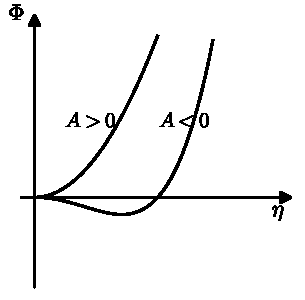
\includegraphics[width=6cm]{fig62.pdf}\\[0.3em]{\small 图 62}\end{minipage}\par\nopagebreak

但是，如果相变点本身是稳定态，即 $\Phi$ 作为 $\eta$ 的函数在这一点（$\eta=0$）有极小值，那里的三次项必须为零，而四次项为正.因此，必须有
\begin{equation}
  A_c(P,T)=0,\quad C_c(P,T)=0,\quad B_c(P,T)>0,
\end{equation}
式中下标c表示相变点.系数B在相变点处为正，当然在该点邻域也为正.

这里存在两种可能情况.由于物体的对称性三次项可能恒为零：$C(P,T)=0$.这时在相变点只剩下一个条件 $A(P,T)=0$；它决定 $P$ 和 $T$ 彼此之间的函数关系.因此，（在PT平面内）存在二级相变点的整条曲线\footnote{但是该条件需要精确化，参看§145第六个脚注.}.

假如C不恒为零，则相变点由两个方程决定：$A(P,T)=0$，$C(P,T)=0$.因此，在这种情形下，连续相变点只可能是孤立点\footnote{可以证明：对于各向同性液体和固态晶体之间的相变，展开式中的三次项总存在.参看 Л.~Д.~Ландау//ЖЭТФ. 1973. Т.~7. С.~627.（文集—第一卷. 第29篇论文，—М.: Наука, 1969.）}.

当然，连续相变点构成一条线的情形更有意思，以下说二级相变也就指这种情况.其中一个特例是与磁结构的出现或消失有关的相变.这种情况是时间反演对称的结果.在这个变换下磁矩（在这里起序参量的作用）变号，而物体的热力学势却不会改变.因此，显然这时 $\Phi$ 的展开式通常不含任何奇次项.

于是，我们假定 $C\equiv0$，而热力学势的展开式具有形式
\begin{equation}
  \Phi(P,T,\eta)=\Phi_0(P,T)+A(P,T)\eta^2+B(P,T)\eta^4.
\end{equation}
式中 $B>0$，而在对称相中 $A>0$，在非对称相中 $A<0$；相变点取决于方程 $A(P,T)=0$.

在这里的理论中已假定函数 $A(P,T)$ 在相变点没有奇点，因此在其附近函数可按偏离该点“距离”的整数幂展开
\begin{equation}
  A(P,T)=a(P)(T-T_c),
\end{equation}
式中 $T_c=T_c(P)$ 是相变温度.系数 $B(P,T)$ 可以用 $B(P)=B(P,T_c)$ 代替.因此，热力学势的展开式取如下形式
\begin{equation}
  \Phi(P,T,\eta)=\Phi_0(P,T)+a(P)(T-T_c)\eta^2+B(P)\eta^4,
\end{equation}
并且 $B(P)>0$.

在非对称相中，在相变点附近 $\eta$ 对温度的依赖关系，取决于 $\Phi$ 作为 $\eta$ 的函数是极小值的条件.令偏微商 $\partial\Phi/\partial\eta$ 等于零，我们得到 $\eta(A+2B\eta^2)=0$，因此
\begin{equation}
  \eta^2=-\frac{A}{2B}=\frac{a}{2B}(T_c-T).
\end{equation}
（$A<0$ 时的根 $\eta=0$ 对应于 $\Phi$ 的极大值，而不是极小值.）应该注意到，两相在温度标尺上的排列与a的符号有关：当 $a>0$ 时，温度 $T<T_c$ 对应于非对称相；而 $a<0$ 时温度 $T>T_c$\footnote{为明确起见，以下总是认定对称相位于 $T>T_c$，这也是绝大多数的情况.相应地，取 $a>0$.}.

忽略 $\eta$ 的高次幂，求得熵
\begin{equation*}
  S=-\frac{\partial\Phi}{\partial T}=S_0-\frac{\partial A}{\partial T}\eta^2
\end{equation*}
（由于 $\partial\Phi/\partial\eta=0$，$\eta$ 对温度的导数项消失）.在对称相中，$\eta=0$，而 $S=S_0$；在非对称相中
\begin{equation}
  S=S_0+\frac{a^2}{2B}(T-T_c).
\end{equation}
正好在相变点上该式变为 $S_0$，因此熵理所当然地保持连续.

最后，我们确定两相在相变点的热容 $C_p=T(\partial S/\partial T)_P$.对于非对称相，(143.7)式求微商得
\begin{equation}
  C_p=C_{p0}+\frac{a^2T_c}{2B}.
\end{equation}
就对称相而言，$S=S_0$，所以 $C_p=C_{p0}$.这样，在二级相变点热容经历跃变.由于 $B>0$，在相变点 $C_p>C_{p0}$，也就是说，从对称相转变到非对称相时热容增加（不问它们的温度顺序）.

除 $C_p$ 以外，经受跃变的还有其它一些量：$C_v$、热膨胀系数、压缩率，等等.不难推导所有这些量跃变间的关系.首先，我们注意到体积和熵在相变点连续，即它们的跃变 $\Delta V$ 与 $\Delta S$ 为零：
\begin{equation*}
  \Delta V=0,\quad\Delta S=0.
\end{equation*}
{\emergencystretch=3em
假定沿相变点曲线压强是温度函数，把这两个等式沿该曲线对温度微分.因为 $(\partial S/\partial P)_T=\allowbreak-(\partial V/\partial T)_P$，结果得
\begin{equation}
  \Delta\Bigl(\frac{\partial V}{\partial T}\Bigr)_P
  +\frac{\mathrm{d}P}{\mathrm{d}T}\Delta\Bigl(\frac{\partial V}{\partial P}\Bigr)_T=0,
\end{equation}
\begin{equation}
  \frac{\Delta C_p}{T}-\frac{\mathrm{d}P}{\mathrm{d}T}
  \Delta\Bigl(\frac{\partial V}{\partial T}\Bigr)_P=0.
\end{equation}
}
这两个方程把热容 $C_p$、热膨胀系数和压缩率在二级相变点的跃变联系起来（V.~Keesom，P.~Ehrenfest，1933）.

以温度和体积作为独立变量，沿相变点曲线求 $\Delta S=0$ 和 $\Delta P=0$（相变时压强不变）的微商，可得
\begin{equation}
  \Delta\Bigl(\frac{\partial P}{\partial T}\Bigr)_V
  +\frac{\mathrm{d}V}{\mathrm{d}T}\Delta\Bigl(\frac{\partial P}{\partial V}\Bigr)_T=0,
\end{equation}
\begin{equation}
  \frac{\Delta C_v}{T}+\frac{\mathrm{d}V}{\mathrm{d}T}
  \Delta\Bigl(\frac{\partial P}{\partial T}\Bigr)_V=0.
\end{equation}
我们注意到，
\begin{equation}
  \Delta C_p=T\Bigl(\frac{\mathrm{d}P}{\mathrm{d}T}\Bigr)^{2}
  \Delta\Bigl(-\frac{\partial V}{\partial P}\Bigr)_T,
\end{equation}
\begin{equation}
  \Delta C_v=-T\Bigl(\frac{\mathrm{d}V}{\mathrm{d}T}\Bigr)^{2}
  \Delta\Bigl(-\frac{\partial V}{\partial P}\Bigr)_T^{-1},
\end{equation}
因而热容的跃变与压缩率的跃变同号.从上述关于热容跃变的结论得出：由非对称相到对称相压缩率跃变地减小.

在本节最后，我们再次回到开头并考虑函数 $\Phi(P,T,\eta)$ 的含义问题.

在形式上引入了任意值 $\eta$ 下的这个函数，这一般并不要求实际上存在与这些值对应的宏观状态（即不完全平衡态）.然而，必须强调，在二级相变点附近，这样的态事实上存在.实际上，随着逼近相变点时，$\Phi$ 作为 $\eta$ 的函数，其极小变得越来越平.这表明使物体达到有平衡值 $\eta$ 状态的“回复力”变得越来越弱，因而关于序参量的平衡建立弛豫时间无限增大（而且总是长于物体建立均等压强的时间）.

\begin{xiti}

求溶液二级相变中比热突变与溶解热突变之间的关系（I.~M.~栗弗席兹，1950）.

解：单溶质分子的溶解热定义为
\begin{equation*}
  q=\frac{\partial W}{\partial n}-w_0',
\end{equation*}
式中W是溶液的焓，而 $w_0'$ 是纯溶质的单分子焓.由于 $w_0'$ 不受溶液中相变所影响，对于 $q$ 的跃变有
\begin{equation*}
  \Delta q=\Delta\frac{\partial W}{\partial n}
  =\Delta\frac{\partial}{\partial n}\Bigl(\Phi-T\frac{\partial\Phi}{\partial T}\Bigr)
  =-T\Delta\frac{\partial^2\Phi}{\partial n\,\partial T}
\end{equation*}
（这里已用到化学势 $\mu'=\partial\Phi/\partial n$ 在相变时连续）.另一方面，把方程 $\Delta(\partial\Phi/\partial T)=0$（熵的连续性）沿相变温度作为浓度c函数的曲线（在压强不变下）求微商，得
\begin{equation*}
  \frac{\mathrm{d}T_c}{\mathrm{d}c}\Delta\frac{\partial^2\Phi}{\partial T^2}
  +N\Delta\frac{\partial^2\Phi}{\partial n\,\partial T}=0.
\end{equation*}
由此得出所求的关系式：
\begin{equation*}
  N\Delta q=\frac{\mathrm{d}T_c}{\mathrm{d}c}\Delta C_p.
\end{equation*}
应该指出，在推导这个关系时没有对溶液的浓度作任何假设.

\end{xiti}

\section{外场对相变的影响}

现在我们考虑：当物体受到外场作用且外场效应依赖于参量 $\eta$ 时，相变的性质如何变化.我们不指定这种场的物理本性，只以普遍形式来表示对场的假设.这就导致，场的作用可描述为在物体的哈密顿算符中出现了如下形式的微扰算符
\begin{equation}
  \hat{H}_h=-\hat{\eta}hV,
\end{equation}
该算符与场的“强度”h和 $\eta$ 量的算符 $\hat{\eta}$ 成线性关系；V是物体的体积\footnote{例如，在铁磁体的居里点（顺磁相的相变点）附近，参量 $\eta$ 是单位体积中的宏观磁矩，而场h是磁场；在铁电体中，参量 $\eta$ 是物体单位体积的电偶极矩，而h是电场.在其它的情形下，场h可能并没有直接的物理含义，但是，形式地引入场有助于加深理解相变的性质.}.假如把热力学势定义为P，T和h的函数，根据参量微商定理（参看(11.4)，(15.11)），$\eta$ 的平均（平衡）值由如下公式给出
\begin{equation}
  V\overline{\eta}=-\frac{\partial\Phi(P,T,h)}{\partial h}.
\end{equation}
为了保证朗道理论中这些关系式成立，展开式(143.5)必须附加上一项 $-\eta hV$：
\begin{equation}
  \Phi(P,T,\eta)=\Phi_0(P,T)+at\eta^2+B\eta^4-\eta hV,
\end{equation}
式中引入了记号 $t=T-T_c(P)$\footnote{在朗道理论中，平衡值 $\eta(P,T)$ 取决于该展开式的极小值，即条件 $\partial\Phi(P,T,\eta)/\partial\eta=0$.当然，关系式(144.2)也满足：$\dfrac{\partial\Phi}{\partial h}=\Bigl(\dfrac{\partial\Phi}{\partial h}\Bigr)_{\eta}+\Bigl(\dfrac{\partial\Phi}{\partial\eta}\Bigr)_{h}\dfrac{\partial\eta}{\partial h}=\Bigl(\dfrac{\partial\Phi}{\partial h}\Bigr)_{\eta}=-V\eta.$}.

首先，我们注意到，场无论多弱都导致在整个温度范围内参量 $\eta$ 变得不为零.换句话说，场降低了高对称相的对称，以致两相之间的差别消失.相应地，孤立相变点也消失；相变被“消解”.特别是比热不再跃变，而是在一整个温度区间内出现反常，该区间的数量级可以从条件 $\eta hV\sim at\eta^2$ 估计出来，$\eta$ 取(143.6)后，得
\begin{equation*}
  t\sim h^{2/3}\frac{B^{1/3}V^{2/3}}{a}.
\end{equation*}
为定量地研究相变，我们写出平衡条件 $(\partial\Phi/\partial\eta)_{T,h}=0$\footnote{我们只考虑在给定压强下的相变：为简单起见，略去表示在求微商时压强不变的下标P.}：
\begin{equation}
  2at\eta+4B\eta^3=hV.
\end{equation}
高于和低于 $T_c$ 的温度下，$\eta$ 与场h的依赖关系不同\footnote{值得提醒，我们约定了 $a>0$，因此对称相（当 $h=0$ 时，$\eta=0$）对应于温度 $t>0$（$T>T_c$）.}.

在 $t>0$ 时，方程(144.4)的左边随 $\eta$ 单调增加（图63a）.因此在每一个给定的h值下，方程只有一个（实）根，它在 $h=0$ 时变为零.函数 $\eta(h)$ 是单值的，并且 $\eta$ 的正负与h完全一致（图64a）.

如果 $t<0$，则方程(144.4)的左边不是 $\eta$ 的单调函数（图63b），因此在h值的一定区间内，方程具有三个不同的实根，函数 $\eta(h)$ 不再是单值的（如图64b所示）.这个区间的边界，显然取决于条件
\begin{equation*}
  \frac{\partial}{\partial\eta}\bigl(2at\eta+4B\eta^3\bigr)=2at+12B\eta^2=0,
\end{equation*}
也就是不等式 $-h_t<h<h_t$，式中
\begin{equation}
  h_t=\Bigl(\frac{2}{3}\Bigr)^{3/2}\frac{(a|t|)^{3/2}}{VB^{1/2}}.
\end{equation}

\par\nopagebreak\noindent\begin{minipage}{\linewidth}\centering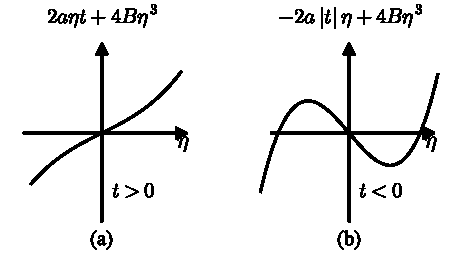
\includegraphics[width=8cm]{fig63.pdf}\\[0.3em]{\small 图 63}\end{minipage}\par\nopagebreak

\par\nopagebreak\noindent\begin{minipage}{\linewidth}\centering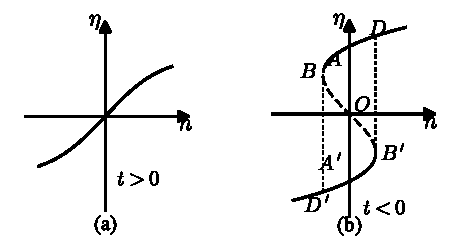
\includegraphics[width=8cm]{fig64.pdf}\\[0.3em]{\small 图 64}\end{minipage}\par\nopagebreak

但是容易看出，$(\partial\eta/\partial h)_T<0$ 的整段曲线 $BB'$，对应于热力学不稳定态.实际上，方程(144.4)对h求微商，得
\begin{equation}
  \Bigl(\frac{\partial\eta}{\partial h}\Bigr)_T
  \Bigl(\frac{\partial^2\Phi}{\partial\eta^2}\Bigr)_{T,h}=V;
\end{equation}
由此看到，当 $(\partial\eta/\partial h)_T<0$ 时，$(\partial^2\Phi/\partial\eta^2)_{T,h}<0$，即在这里 $\Phi$ 有极大，而非极小.

在曲线段AB和 $A'B'$ 上，热力学势为极小，但是这种极小值分别大于曲线段 $A'D'$ 和AD对应的极小值；这由直接计算容易证实，然而结果也显然可以预见：因为场h以 $-\eta hV$ 项出现在 $\Phi$ 中，$\eta$ 与h同号必定在热力学上有利.换而言之，曲线段AB和 $A'B'$ 对应于物体的亚稳态.因此，函数 $\eta(h)$ 的真实平衡行为由图64b所示的连续线段 $DAA'D'$ 给出，线上所有的点对应于热力学稳态.如果在给定的温度 $t<0$ 下改变场，则在经过值 $h=0$ 时出现一级相变：值反号的 $\eta=\pm\bigl(\frac{a|t|}{2B}\bigr)^{1/2}$ 的两相在该点彼此处于平衡.

物体的磁化率定义为导数
\begin{equation}
  \chi=\Bigl(\frac{\partial\eta}{\partial h}\Bigr)_{T:h=0}.
\end{equation}
对等式(144.4)求微商，得
\begin{equation*}
  \frac{\partial\eta}{\partial h}=\frac{V}{2at+12B\eta^2};
\end{equation*}
当 $h\to0$ 时对于 $t>0$ 有 $\eta^2=0$ 且对于 $t<0$ 有 $\eta^2=-\frac{at}{2B}$，代入上式得
\begin{equation}
  \chi=\frac{V}{2at}\ \text{当}\ t>0\ \text{时，}\qquad
  \chi=\frac{V}{-4at}\ \text{当}\ t<0\ \text{时.}
\end{equation}
当 $t\to0$ 时 $\chi$ 变为无穷大，这个结果很自然：正如在上节最后所述，随着相变点的趋近，函数 $\Phi(\eta)$ 的极小变得越来越平；正因为如此，即使不大的微扰也强烈地影响 $\eta$ 的平衡值.

如果场的大小取以下值
\begin{equation*}
  h_t\sim\frac{(a|t|)^{3/2}}{VB^{1/2}},
\end{equation*}
则场所诱发的参量 $\eta_{\mathrm{ind}}\sim\chi h$ 与自发的（无场）特征量 $\eta_{\mathrm{sp}}\sim(a|t|/B)^{1/2}$ 同样数量级.场 $h\ll h_t$ 是“弱的”，意味着在一级近似下场不影响物体的热力学量.场 $h\gg h_t$ 形成“强场”区，其中热力学量的值在一级近似下取决于场；显然当 $t=0$ 时，任何场在此意义下都是强场.

在强场区，序参量
\begin{equation}
  \eta=\Bigl(\frac{hV}{4B}\Bigr)^{1/3}.
\end{equation}
容易验证：在此区热容 $C_p$ 与场的大小无关.

\section{二级相变中对称的改变}

在上几节所讨论的理论中，我们考虑了物体的对称发生一定改变的二级相变，预先假定这样的相变是可能的.但是，这样的理论不可能回答，对称的改变实际上究竟是否通过二级相变发生.本节将细述的理论就是为了这个目的，它的出发点是问题的另一种提法：物体在相变点处的特定对称给定后，回答在该点两侧可能有何种对称.

为了明确起见，我们讨论由晶格结构改变亦即晶格中原子位形对称的改变所引起的相变.设 $\rho(x,y,z)$ 为（在§128中引入的）密度函数，它决定晶体中原子在不同位置的概率分布.晶格的对称是那些使函数 $\rho(x,y,z)$ 保持不变的坐标变换的集合（群）.自然，这里是指晶格的全部对称，包括旋转、反映以及所有可能平行位移（平移）的无限（离散）集合；换句话说，是230个空间群中的一个.

设 $G_0$ 为晶体在相变点处的对称群.由群论知道，任意函数 $\rho(x,y,z)$ 可以用某些函数 $\varphi_1,\varphi_2,\cdots$ 的线性组合来表示，这些函数具有可在给定群的所有变换下相互转换的性质.在一般情形下，这些函数的数目等于该群元素的数目；但是如果被展开的函数 $\rho$ 本身具有一定的对称，那么函数 $\varphi_i$ 的数目也可能较少.

考虑到这一点，晶体的密度函数 $\rho(x,y,z)$ 可表示成和式
\begin{equation*}
  \rho=\sum_i\eta_i\varphi_i,
\end{equation*}
式中函数 $\varphi_i$ 在群 $G_0$ 的所有变换下相互变换.这些变换的矩阵构成群 $G_0$ 的所谓表示.函数 $\varphi_i$ 的选择不唯一；显然，可以用它们的任何线性组合来代替它们本身.大家知道，总是可以适当选择函数 $\varphi_i$，以使得它们可分成几组，每组包含数目尽可能少的函数，并且在群 $G_0$ 的所有变换下构成每组的函数只在组内相互变换.这些组中每组函数的变换矩阵是群 $G_0$ 的不可约表示，而这些函数本身是表示的基.因此，可写
\begin{equation}
  \rho=\sum_n\sum_i\eta_i^{(n)}\varphi_i^{(n)},
\end{equation}
式中n是不可约表示的编号，i是它的基函数编号.以下假定函数 $\varphi_i^{(n)}$ 已以某种方式归一化了.

在函数 $\varphi_i^{(n)}$ 中，总有一个它本身在群 $G_0$ 的所有变换下不变（构成群的单位表示）.换句话说，这个函数（记作 $\rho_0$ 来代表）具有 $G_0$ 的对称.把 $\rho$ 的其余部分用 $\delta\rho$ 来表示，可写
\begin{equation}
  \rho=\rho_0+\delta\rho,\quad
  \delta\rho=\sum_n'\sum_i\eta_i^{(n)}\varphi_i^{(n)},
\end{equation}
式中已经把群的单位表示排除在求和之外（这用带撇的求和号表示）.

函数 $\delta\rho$ 具有比 $G_0$ 低的对称，因为即使 $\delta\rho$ 在这个群的某些变换下保持不变，也总不会在所有变换下都如此.我们注意到，函数 $\rho$ 的对称G（显然同 $\delta\rho$ 的对称一致），严格地说，从一开始就假定低于对称 $G_0$，否则，整个和式(145.1)就会只有一项即构成单位表示的函数 $\rho$ 本身\footnote{对于磁相变，代替密度 $\rho(x,y,z)$ 必须考虑物体中的电流密度 $\boldsymbol{j}(x,y,z)$.在顺磁相中 $\boldsymbol{j}=0$，而在相变点的另一侧 $\boldsymbol{j}=\delta\boldsymbol{j}$ 很小.}.

因为物理量 $\delta\rho$ 是实的，而且在所有的变换下仍应如此，说到不可约表示，显然应该指物理上的不可约表示，其基函数可以取实函数（§135）；与此相应，以后假定函数 $\varphi_i^{(n)}$ 总是实的.

晶体的热力学势 $\Phi$ 是密度函数 $\rho$ 的泛函，并且以参量的形式依赖于压强P和温度T
\begin{equation*}
  \Phi=\Phi\{\rho;P,T\}.
\end{equation*}
换句话说，$\Phi$ 是诸系数 $\eta_i^{(n)}$ 的函数（当然依赖于函数 $\varphi_i^{(n)}$ 本身的具体形式）.

$\eta_i^{(n)}$ 作为P和T的函数的实际取值由热力学平衡条件即 $\Phi$ 为极小条件来决定.于是，晶体的对称G也被确定，因为函数(145.2)的对称显然取决于函数 $\varphi_i^{(n)}$ 线性组合中系数的值，而 $\varphi_i^{(n)}$ 的变换规律已知.

为保证晶体在相变点处具有对称 $G_0$，必须使全部的 $\eta_i^{(n)}$ 在该点变为零，即 $\delta\rho=0$，$\rho=\rho_0$.因为晶体在二级相变时状态的变化是连续的，所以 $\delta\rho$ 在相变点也应该连续而无跳跃地变为零，即系数 $\eta_i^{(n)}$ 必须趋于零且在相变点附近可取任意小的值.因而，热力学势 $\Phi(P,T,\eta_i^{(n)})$ 在相变点附近可展成 $\eta_i^{(n)}$ 的幂级数.

我们首先指出，在群 $G_0$ 的变换下函数 $\varphi_i^{(n)}$ 相互变换（在每个不可约表示的基函数内），因此可以用另一种方式表示这些变换；仿佛是系数 $\eta_i^{(n)}$ 按同样规律被变换，而不是函数 $\varphi_i^{(n)}$.其次，因为物体的热力学势显然不会依赖于坐标系的选择，所以它相对于坐标系的任何变换一定是不变的.

如果某个变换把 $\rho_0$ 变为 $\rho_0'$，而 $\delta\rho$ 变为 $\delta\rho'$，则
\begin{equation*}
  \Phi\{\rho_0+\delta\rho\}=\Phi\{\rho_0'+\delta\rho'\}.
\end{equation*}
由此可见，如果把势看成在给定 $\rho_0$ 下只是 $\delta\rho'$ 的泛函，则对于不改变 $\rho$ 的变换即 $G_0$ 群的变换，$\Phi$ 是不变的.因此在 $\Phi$ 的 $\eta_i^{(n)}$ 幂展开中，每一项应该只包含适当幂次的 $\eta_i^{(n)}$ 的不变组合.

按照群的不可约表示（非单位表示）变换的量，构不成线性不变式\footnote{否则意味着在给定的表示中含有单位表示，即表示是可约的.}.然而，每个表示却有唯一的二次不变式，即 $\eta_i^{(n)}$ 的正定二次型，它总可以化成平方和.

因此，$\Phi$ 展开式始于如下形式：
\begin{equation}
  \Phi=\Phi_0+\sum_n'A^{(n)}\sum_i\eta_i^{(n)2},
\end{equation}
式中 $A^{(n)}$ 是P和T的函数.

在相变点上，晶体必须具有对称 $G_0$，就是说，值 $\eta_i^{(n)}=0$ 应该对应于平衡态.显然，只有在所有的 $A^{(n)}$ 非负时，$\Phi$ 才可能当全部 $\eta_i^{(n)}=0$ 时有极小值.

如果在相变点处所有的 $A^{(n)}>0$，则在相变点附近它们也是正的，也就总有 $\eta_i^{(n)}=0$，因而根本不会发生任何对称变化.为使非零的 $\eta_i^{(n)}$ 出现，系数 $A^{(n)}$ 之一必须变号；因此在相变点处这个系数应该变为零\footnote{更确切地说，这个条件应该表述如下.诸系数 $A^{(n)}$ 当然依赖于函数 $\varphi_i^{(n)}$ 的具体形式，它们是这些以P和T作为参量的函数的二次泛函.在相变点的一侧，所有这些泛函 $A^{(n)}\{\varphi_i^{(n)};P,T\}$ 实质上是正的.相变点可定义为这样一点：在该点（随着P或T的缓慢改变），$A^{(n)}$之一可以为零：$A^{(n)}\{\varphi_i^{(n)};P,T\}\geqslant0$.这个为零条件对应于特定的一组函数 $\varphi_i^{(n)}$，原则上它们可以由求解适当的变分问题来确定.这些函数也是确定在相变点处变化 $\delta\rho$ 的函数 $\varphi_i^{(n)}$.把它们代入泛函 $A^{(n)}\{\varphi_i^{(n)};P,T\}$，正好得到函数 $A^{(n)}(P,T)$，后者在相变点处满足条件 $A^{(n)}(P,T)=0$.此后可以认为函数 $\varphi_i^{(n)}$ 已经给定，后面也总这样假定.（允许 $\varphi_i^{(n)}$ 随P和T变，会导致阶次比这里考虑各项高的修正项.）}.（两个系数 $A^{(n)}$ 同时变成零的情况只能发生在PT平面的孤立点上.这样的点是多条二级相变曲线的交点.）

于是，在相变点的一侧，所有的 $A^{(n)}>0$，而在另一侧系数 $A^{(n)}$ 之一为负.与此相应，在相变点的一侧，总是所有的 $\eta_i^{(n)}=0$，而在另一侧出现非零的 $\eta_i^{(n)}$.换而言之，可以下结论：在相变点的一侧，晶体具有较高的对称 $G_0$，这种对称维持至相变点处，而在相变点的另一侧，对称降低，因而群G是群 $G_0$ 的子群.

由于 $A^{(n)}$ 之一变号，出现了属于相应的第n个表示的非零 $\eta_i^{(n)}$.因此，具有对称 $G_0$ 的晶体变成密度为 $\rho=\rho_0+\delta\rho$ 的晶体，此处
\begin{equation}
  \delta\rho=\sum_i\eta_i^{(n)}\varphi_i^{(n)}
\end{equation}
是群 $G_0$ 的单个不可约表示（任何非单位表示）基函数的线性组合.以下略去不可约表示编号的角标n，而总是指恰巧出现在所考虑相变中的那个.

我们引入记号
\begin{equation}
  \eta^2=\sum_i\eta_i^2,\quad\eta_i=\eta\gamma_i
\end{equation}
（因而 $\sum_i\gamma_i^2=1$），并把 $\Phi$ 的展开式写成
\begin{equation}
\begin{aligned}
  \Phi={}&\Phi_0(P,T)+\eta^2A(P,T)
  +\eta^3\sum_\alpha C_\alpha(P,T)f_\alpha^{(3)}(\gamma_i)+{}\\
  &+\eta^4\sum_\alpha B_\alpha(P,T)f_\alpha^{(4)}(\gamma_i)+\cdots,
\end{aligned}
\end{equation}
式中 $f_\alpha^{(3)},f_\alpha^{(4)},\cdots$ 是由诸 $\gamma_i$ 构成的三次、四次等阶次不变式；对于每一阶次由 $\gamma_i$ 可以构成多少个独立的不变式，则相应的对 $\alpha$ 求和就有多少项.在热力学势的这个展开式中，系数A在相变点必须变成零.为使相变点本身是稳态（即在 $\eta_i=0$ 时 $\Phi$ 在该点具有极小值），三次项必须为零，而四次项必须实质上为正.在§143中已经指出，只有在 $\Phi$ 的展开式中三次项恒为零的条件下，二级相变曲线（在PT平面中）才能够存在.现在可以把上述条件表述为：如果 $\eta_i$ 按照群 $G_0$ 的给定不可约表示变换，用这些量不可能构成三次不变式\footnote{用表示论的语言说，这表明给定表示 $\Gamma$ 的所谓对称立方 $[\Gamma^3]$ 本身不应该含有单位表示.对于空间群的不可约（字面意义上）表示，三次不变式不可能多于一个（其证明参看：Шур М.~С. // ЖЭТФ. 1966. Т.~51. С.~1260）.把两个表示合并为一个物理上不可约表示时，可能出现两个三次不变式.}.

假设这个条件被满足，精确到四次项的展开式可写成
\begin{equation}
  \Phi=\Phi_0+A(P,T)\eta^2+\eta^4\sum_\alpha B_\alpha(P,T)f_\alpha^{(4)}(\gamma_i).
\end{equation}
因为二次项不含 $\gamma_i$，所以这些量直接由四次项即(145.7)中 $\eta^4$ 的系数为极小的条件来决定\footnote{有可能四次不变式只一个 $\bigl(\sum_i\eta_i^2\bigr)^2=\eta^4$.这种情形下，四次项不依赖于 $\gamma_i$，必须用依赖于 $\gamma_i$ 的高次项来定 $\gamma_i$.在某些情形下，如果依赖于 $\gamma_i$ 的四次项求极小后变为零，也有必要计算高次项.}.把这个系数相应的极小值直接记为 $B(P,T)$（根据以上所述，它必须为正），我们得到形为(143.3)的 $\Phi$ 展开式，而将 $\Phi$ 看作只是 $\eta$ 的函数，像在§143中所做的那样，由 $\Phi$ 为极小的条件可决定 $\eta$.这样求出的 $\gamma_i$ 值决定函数 $\delta\rho$ 的对称：
\begin{equation}
  \delta\rho=\eta\sum_i\gamma_i\varphi_i,
\end{equation}
即确定了对称为 $G_0$ 的晶体在二级相变后所形成的对称G\footnote{在§143中，我们考虑了具有给定对称变化的相变.用这里所引入的概念，可以说我们事先假定了 $\gamma_i$ 这些量具有给定的值（因而函数 $\delta\rho$ 有给定的对称）.在这样表述问题时，在展开式(143.3)中不出现三次项，这不会是保证存在二级相变点曲线的充分条件，因为它并不排除在用几个 $\gamma_i$ 展开的普遍式中出现三次项的可能性（如果给定的不可约表示非一维）.例如，如果有三个 $\eta_i$ 量，并且乘积 $\gamma_1\gamma_2\gamma_3$ 是不变式，则 $\Phi$ 的展开式含三次项，然而，当函数 $\delta\rho$ 具有特定对称从而要求一个或两个 $\gamma_i$ 为零时这个三次项变成零.}.

在上述形式下，$\eta_i$ 这些量的集合起序参量的作用，描述非对称相偏离对称相的程度.我们看到，这个参量一般是多分量的，并且比值 $\gamma_i=\eta_i/\eta$ 确定非对称相的对称，而公因子 $\eta$ 定量地度量对给定对称的偏离.

但是，所得出的条件还不足以保证二级相变能够存在.如果考虑到与空间群表示的分类性质有关的事实\footnote{本节下面所叙述的结果与例子由 E.~M.~栗弗席兹（1941）得出.}（至今有意未提到），还有一个重要的条件需要阐明.在§134中已看到，这些表示不仅按离散的特征（如小表示的编号）分类，而且还按取一系列连续值的参量k分类.因而在展开式(145.3)中系数 $A^{(n)}$ 应该不仅依赖于离散编号n，而且也依赖于连续变量k.

设相变与系数 $A^{(n)}(k)$（作为P和T的函数）变为零有关，这个系数具有确定编号n和确定值 $k=k_0$.但是，为使相变实际上发生，必须使 $A^{(n)}$ 作为k的函数在 $k=k_0$ 处（从而在 $k_0$ 波矢星的所有矢量处）有极小值，即 $A^{(n)}(k)$ 在 $k_0$ 的附近按 $k-k_0$ 的展开式应不含线性项.否则，某些系数 $A^{(n)}(k)$ 必定会先于 $A^{(n)}(k_0)$ 变为零，所考虑类型的相变便不可能发生.根据以下讨论，可以得到这个条件的方便表述.

值 $k_0$ 确定函数 $\varphi_i$ 的平移对称，因而也确定函数 $\delta\rho$(145.8)的平移对称即新相的晶格周期.这个结构应该比k值在 $k_0$ 附近的结构稳定.但是 $k=k_0+\varkappa$（$\varkappa$ 为小量）的结构与 $k=k_0$ 的结构相差一个后者周期的空间“调制”，即在比晶格周期（胞线度）大许多的距离（$\sim1/\varkappa$）上出现不均匀性.这种不均匀性的宏观描述，是将序参量 $\eta_i$ 当作缓变的坐标函数（而 $\eta_i\varphi_i$ 在原子间的距离上振荡）.因而，我们得出晶体状态相对于宏观均匀性破坏的稳定性要求.

量 $\eta_i$ 在空间上非恒定时，晶体热力学势密度不仅依赖于 $\eta_i$，而且还依赖于其坐标微商（在一级近似下依赖于一阶微商）.与此相应，在相变点附近，必须把 $\Phi$（每单位体积）按 $\eta_i$ 及其梯度 $\nabla\eta_i$ 的幂展开.如果（整个晶体的）热力学势在常数 $\eta_i$ 下应取极小，这个展开式中梯度一次项应恒为零（微商的二次项应该是正定的；但是这个情况对 $\eta_i$ 并不施加任何限制，因为对于按照任何不可约表示变换的 $\eta_i$，这样的二次型存在）.

在微商的线性项中，较重要的只是正比于 $\partial\eta_i/\partial x,\cdots$ 的项以及含乘积 $\eta_i\partial\eta_k/\partial x,\cdots$ 的项.高次项显然不重要.整个晶体的热力学势即全体积积分 $\int\Phi\,\mathrm{d}V$ 应取极小.但是 $\Phi$ 中所有的全微商在积分后给出常数，对积分极小的决定无影响；因而可以略去 $\Phi$ 中只与 $\eta_i$ 的微商成正比的所有项.在含乘积 $\eta_i\partial\eta_k/\partial x,\cdots$ 的项中，可以略去所有对称组合
\begin{equation*}
  \eta_k\frac{\partial\eta_i}{\partial x}
  +\eta_i\frac{\partial\eta_k}{\partial x}
  =\frac{\partial}{\partial x}\eta_i\eta_k,\cdots,
\end{equation*}
只保留反对称的部分
\begin{equation}
  \eta_k\frac{\partial\eta_i}{\partial x}
  -\eta_i\frac{\partial\eta_k}{\partial x},\cdots
\end{equation}
在 $\Phi$ 的展开式中只能有(145.9)量的不变线性组合.所以，出现相变的可能性条件是不存在这样不变量\footnote{这样不变量称为栗弗席兹不变量.}.

梯度 $\nabla\eta_i$ 的分量，像矢量分量与 $\eta_i$ 的乘积一样变换.因此，差(145.9)变换时如同矢量分量再乘以量 $\eta_i$ 的反对称积.于是，要求由(145.9)量不可能构成一个线性标量，等效于要求不可能由反对称积
\begin{equation}
  \chi_{ik}=\varphi_i\varphi_k'-\varphi_k\varphi_i'
\end{equation}
构成任何组合而可像一个矢量分量那样变换（这里 $\varphi_i,\varphi_i'$ 是相应不可约表示的同样基函数，为避免差恒等于零，它们取在两个不相同的点 $x,y,z$ 和 $x',y',z'$ 上）.\footnote{在表示理论中这表明，给定表示 $\Gamma$ 的反对称平方 $\{\Gamma^2\}$ 不应该包含矢量分量变换所遵从的不可约表示.}用两个指标 $k\alpha$ 标记表示的基函数（如§134），我们把差(145.10)写成
\begin{equation}
  \chi_{k\alpha,k'\beta}
  =\varphi_{k\alpha}\varphi_{k'\beta}'
  -\varphi_{k\alpha}'\varphi_{k'\beta},
\end{equation}
式中 $k,k',\cdots$ 是同一波矢星的矢量.

设矢量k占据最一般的位置而且没有任何纯对称.按照旋转群元的数目，波矢星k含有n个矢量（如果空间群自身不含反演，则为2n个），并且每个k都伴有与之不同的矢量$-$k.相应的不可约表示由相同数目的函数 $\varphi_k$（每k一个，因而略去角标 $\alpha$）来实现.量
\begin{equation}
  \chi_{k,-k}=\varphi_k\varphi_{-k}'-\varphi_k'\varphi_{-k}
\end{equation}
在平移下不变.在旋转元素的作用下，这n（或2n）个量相互变换，实现相应点群（晶类）的表示，其维数等于群阶.但是这样的表示（所谓正则表示）含有全部的不可约群表示，其中包括矢量分量变换的表示.

类似的讨论指出，矢量k的群含有一根对称轴和过该轴的对称平面时，有可能由 $\chi_{k\alpha,k\beta}$ 量构造出一个矢量.

但是，如果矢量k的群含有彼此相交的对称轴或与对称面相交的对称轴，或者含有反演（我们说这样的群具有中心点），则上述讨论不适用了.在这种情况下，是否可由(145.11)量构成矢量的问题，必须就具体情况分别处理.特别是，如果k的群含有反演（因而k与$-$k等效），只有一个函数 $\varphi_k$ 对应于波矢星的每个k，则肯定不可能构造这样的矢量：这时不存在 $\chi_{kk'}$ 是平移不变的，而矢量 $\chi_{kk'}$ 分量却总必须这样.

由此可见，所提出的要求大大限制了在二级相变时可能的对称变化.所有无穷多个不同的不可约群表示 $G_0$ 中，只需要考虑为数不多的有中心点的k矢量群.

当然，只有在倒格子中占据某些特殊位置的矢量k，可能有这类纯对称；它们的分量等于倒格子基本周期的某几个简单分数 $\bigl(\frac{1}{2},\frac{1}{3},\frac{1}{4}\bigr)$.这表明，在二级相变下晶体平移对称（即布拉维格子）的变化只可能是某几个基本周期增加不大的倍数.研究证实，在大多数情况下，布拉维格子可能发生的改变是周期加倍.此外，在体心（斜方、四方、立方）晶格和面心立方晶格中某些周期可能有四倍的改变；而在六方晶格中增到三倍.同时，原胞的体积可能增到2,4,8倍；在面心立方晶格中还有增到16或32倍的情形，而在六方晶格中增到3或6倍.

自然，布拉维格子不变的相变也是可能的（$k=0$ 的不可约表示相应于此）.这时对称的变化在于旋转元素数目的减少，即改变晶类.

我们指出如下普遍的定理：对于对称变换数目减半的任何结构变化，二级相变都可能存在；出现这种变化的方式，或是晶类不变而晶体原胞增大一倍，或是原胞不变而旋转和反映的数目减半.证明的依据在于：如果群 $G_0$ 有阶数减半的子群G，则在 $G_0$ 的不可约表示中总有一个一维表示，而实现该表示的函数对于子群G的所有变换不变，但在 $G_0$ 群的所有其余变换下变号.显然，在这种情况下没有奇次不变式，而(145.11)型的量完全不可能由一个函数构成.

可以看出，下面的定理也成立：对于对称变换数目减为三分之一的结构变化，二级相变不可能出现，因为 $\Phi$ 的展开式中存在三次项.

最后，作为上述一般理论的应用实例，我们考虑合金中有序的出现，在无序态中合金具有体心立方晶格，原子位于立方胞的顶点和体心（如图61b所示）\footnote{这种晶格属于点式空间群 $O_h^9$.}.问题在于决定二级相变时这种晶格可出现的可能排序类型（即结晶学中的所谓超晶格）.

对于体心立方晶格，倒格子是面心立方.选取正格子立方胞的棱作为长度单位，则倒格子立方胞的棱长等于 $2\cdot2\pi$.在这个倒格子中，下列矢量k有含中心点的纯对称群：
\begin{equation}
\left.\begin{aligned}
  &\text{(a)}\ \ (0\ 0\ 0)\ \ O_h,\\
  &\text{(b)}\ \ \Bigl(\tfrac{1}{2}\ \tfrac{1}{2}\ \tfrac{1}{2}\Bigr)\ \ O_h,\\
  &\text{(c)}\ \ \Bigl(\tfrac{1}{4}\ \tfrac{1}{4}\ \tfrac{1}{4}\Bigr),\
  \Bigl(-\tfrac{1}{4}\ -\tfrac{1}{4}\ -\tfrac{1}{4}\Bigr)\ \ T_d,\\
  &\text{(d)}\ \ \Bigl(0\ \tfrac{1}{4}\ \tfrac{1}{4}\Bigr),\
  \Bigl(\tfrac{1}{4}\ 0\ \tfrac{1}{4}\Bigr),\
  \Bigl(\tfrac{1}{4}\ \tfrac{1}{4}\ 0\Bigr),\\
  &\qquad\ \Bigl(0\ \tfrac{1}{4}\ -\tfrac{1}{4}\Bigr),\
  \Bigl(-\tfrac{1}{4}\ 0\ \tfrac{1}{4}\Bigr),\
  \Bigl(\tfrac{1}{4}\ -\tfrac{1}{4}\ 0\Bigr)\ \ D_{2h}.
\end{aligned}\right\}
\end{equation}
这里所列的是矢量k在沿倒格子立方胞三条棱方向（$x,y,z$ 轴）上的分量，以棱长为单位度量；如果用上面所选单位写出矢量k，这些数字必须乘以 $2\cdot2\pi=4\pi$.在(145.13)中，只列出不等价的矢量，即每个波矢星k的矢量.

解决所提出的问题时不必考虑所有的小表示，这大大简化了下一步研究.理由在于我们感兴趣只是形成超晶格时可能出现的对称变化，这时原子在现有的格点上有序排列而无相对位移.这种情况下，无序晶格的原胞只含一个原子.因而，超晶格的出现只能是由于不同原胞格点不再等价.这意味着，密度分布函数所产生的变化 $\delta\rho$ 相对于k群的所有旋转变换（不伴有平移）应该不变；换句话说，只允许单位小表示.与此相应，在基函数(134.3)中可以用1代替 $u_\alpha$.

现在我们依次考虑在(145.13)中列举的波矢星k.

a) $k=0$ 的函数有完全的平移不变性.换句话说，在这种情况下原胞不变，而因为每胞只含一个原子，不发生任何对称改变.

b) 与这个k对应的函数是 $\exp[2\pi\mathrm{i}(x+y+z)]$.这个函数以及由之通过所有的旋转和反映所得到的函数可组成线性组合
\begin{equation}
  \varphi=\cos2\pi x\cos2\pi y\cos2\pi z,
\end{equation}
它具有群k的对称 $O_h$.生成相的对称是密度函数 $\rho=\rho_0+\delta\rho$ 的对称，此处 $\delta\rho=\eta\varphi$\footnote{当然，这并不意味着在实际晶体中变化 $\delta\rho$ 就是由函数(145.14)给出.在表达式(145.14)中重要的只是它的对称性.}.函数 $\varphi$ 对于晶类 $O_h$ 的所有变换以及沿立方胞任意一条棱的平移都是不变的，而对于沿空间对角线一半 $\bigl(\frac{1}{2}\ \frac{1}{2}\ \frac{1}{2}\bigr)$ 的平移却不是.因此，有序相有简单立方的布拉维格子且原胞中有两个不等效点：$(0\ 0\ 0)$ 和 $\bigl(\frac{1}{2}\ \frac{1}{2}\ \frac{1}{2}\bigr)$，由不同原子占据.能够按这种形式完全排序的合金，其组成为AB（如§142中所述的合金CuZn）.

c) 与这些矢量k对应的是对称为 $T_d$ 的函数：
\begin{equation}
  \varphi_1=\cos\pi x\cos\pi y\cos\pi z,\quad
  \varphi_2=\sin\pi x\sin\pi y\sin\pi z.
\end{equation}
从这两个可以构成两个四次不变式：$(\varphi_1^2+\varphi_2^2)^2$ 和 $(\varphi_1^4+\varphi_2^4)$.因此 $\Phi$ 的展开式(145.7)形为
\begin{equation}
  \Phi=\Phi_0+A\eta^2+B_1\eta^4+B_2\eta^4\bigl(\gamma_1^4+\gamma_2^4\bigr).
\end{equation}
这里必须区分两种情况.设 $B_2<0$，那么 $\Phi$ 作为 $\gamma_1$ 和 $\gamma_2$ 的函数，在附加条件 $\gamma_1^2+\gamma_2^2=1$ 下有极小点 $\gamma_1=1$，$\gamma_2=0$.函数 $\delta\rho=\eta\varphi_1$ 有面心布拉维格子的晶类 $O_h$ 对称，该晶格立方胞的体积为原来晶格立方胞的8倍.原胞含有四个原子（而立方胞含16个原子）.把同种原子放在等效格点上，借此可以得出，这种超晶格对应于组成为 $ABC_2$ 的三元合金，其原子位置为：

\begin{flushleft}
\hspace{2em}4A\quad $(0\,0\,0)$，$\bigl(0\,\frac{1}{2}\,\frac{1}{2}\bigr)$和循环置换，\\
\hspace{2em}4B\quad $\bigl(\frac{1}{2}\,\frac{1}{2}\,\frac{1}{2}\bigr)$，$\bigl(0\,0\,\frac{1}{2}\bigr)$和循环置换，\\
\hspace{2em}8C\quad $\bigl(\frac{1}{4}\,\frac{1}{4}\,\frac{1}{4}\bigr)$，$\bigl(\frac{3}{4}\,\frac{3}{4}\,\frac{3}{4}\bigr)$，$\bigl(\frac{1}{4}\,\frac{3}{4}\,\frac{3}{4}\bigr)$和循环置换，$\bigl(\frac{1}{4}\,\frac{1}{4}\,\frac{3}{4}\bigr)$和循环置换.
\end{flushleft}

（这里给出的原子坐标，其单位取新立方胞的棱长，为原始胞棱长的两倍；参看图65）.如果原子B和C同种，得到组成为 $AB_3$ 的有序晶格.

现在，设 $B_2>0$.这时在 $\gamma_1^2=\gamma_2^2=1/2$ 处 $\Phi$ 有极小，因此 $\delta\rho=\eta(\varphi_1+\varphi_2)/\sqrt{2}$（或者 $\delta\rho=\eta(\varphi_1-\varphi_2)/\sqrt{2}$，结果相同）\footnote{在两种情形下 $\gamma_1$ 和 $\gamma_2$ 只不过是数，这是由于 $\Phi$ 中只有一项（依赖于 $\gamma_1,\gamma_2$）.如果有多个不同的四次不变式，则使 $\Phi$ 取极小的一组 $\gamma_i$ 中某些会依赖于P，T.}.该函数的对称，与前一种情况同样，属于面心布拉维格子的晶类 $O_h$，但是只有两套等效格点，可分别被A,B两种原子占据：

\begin{flushleft}
\hspace{2em}8A\quad $(0\,0\,0)$，$\bigl(\frac{1}{4}\,\frac{1}{4}\,\frac{1}{4}\bigr)$，$\bigl(\frac{1}{4}\,\frac{3}{4}\,\frac{3}{4}\bigr)$和循环置换，$\bigl(0\,\frac{1}{2}\,\frac{1}{2}\bigr)$和循环置换，\\
\hspace{2em}8B\quad $\bigl(\frac{1}{2}\,\frac{1}{2}\,\frac{1}{2}\bigr)$，$\bigl(\frac{3}{4}\,\frac{3}{4}\,\frac{3}{4}\bigr)$，$\bigl(\frac{1}{4}\,\frac{1}{4}\,\frac{3}{4}\bigr)$和循环置换，$\bigl(0\,0\,\frac{1}{2}\bigr)$和循环置换
\end{flushleft}

（参看图65b）.

\par\nopagebreak\noindent\begin{minipage}{\linewidth}\centering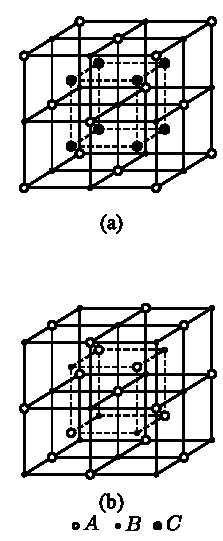
\includegraphics[width=8cm]{fig65.pdf}\\[0.3em]{\small 图 65}\end{minipage}\par\nopagebreak

d) 与这些矢量k对应的是下列函数
\begin{equation*}
\begin{aligned}
  \varphi_1&=\cos\pi(y-z),\qquad
  \varphi_3=\cos\pi(x-y),\qquad
  \varphi_5=\cos\pi(x-z),\\
  \varphi_2&=\cos\pi(y+z),\qquad
  \varphi_4=\cos\pi(x+y),\qquad
  \varphi_6=\cos\pi(x+z).
\end{aligned}
\end{equation*}
它们具有所要求的对称 $D_{2h}$，由这些函数可以构成一个三次不变式和四个四次不变式，因此展开式(145.6)取形式
\begin{equation*}
\begin{aligned}
  \Phi=\Phi_0&+A\eta^2+C\eta^3\bigl(\gamma_1\gamma_3\gamma_5
  +\gamma_2\gamma_3\gamma_6+\gamma_1\gamma_4\gamma_6
  +\gamma_2\gamma_4\gamma_5\bigr)+B_1\eta^4+{}\\
  &+B_2\eta^4\bigl(\gamma_1^4+\gamma_2^4+\gamma_3^4+\gamma_4^4
  +\gamma_5^4+\gamma_6^4\bigr)
  +B_3\eta^4\bigl(\gamma_1^2\gamma_2^2+\gamma_3^2\gamma_4^2
  +\gamma_5^2\gamma_6^2\bigr)+{}\\
  &+B_4\eta^4\bigl(\gamma_1\gamma_2\gamma_3\gamma_4
  +\gamma_3\gamma_4\gamma_5\gamma_6+\gamma_1\gamma_2\gamma_5\gamma_6\bigr).
\end{aligned}
\end{equation*}
由于有立方项，在这种情况下二级相变不可能出现.要考察孤立的连续相变点（参看§150）是否存在及其性质如何，则必须研究函数 $\Phi$ 在其极小值附近的行为，我们不在此继续探讨.

从上一例子我们看到，热力学理论对二级相变的可能性加了非常严格的限制；对于例子中的情形，只能通过形成三种超晶格而实现相变.

值得指出以下的细节：在情形(c)中，$B_2<0$ 时密度函数的实际改变 $\delta\rho=\eta\varphi_1$ 只涉及出现在热力学势(145.16)中的两个参量 $\gamma_1$ 和 $\gamma_2$ 之一.这体现了上述理论的一个重要特征：在研究晶格在二级相变中的具体改变时，也必须考虑“几乎可能”的其它改变.

到目前为止，我们考察了结构对应于矢量k位于倒格子中某个具有有理指标的对称点时的二级相变.这时非对称相像对称相一样有严格的周期性.

另一种情况发生于相变到无公度相时，这种相在§133的末尾曾提及.在这种情形下，k并不对应于倒格子中某个对称点.该矢量可能占据某个对称轴或对称平面上的普通位置，或者空间中的普通位置.对于这种相变，不存在导数线性不变式的要求可以放宽.

假定k位于某个对称轴上.于是问题中存在附加的自由参量——矢量k沿着这个轴的分量 $k_x$.假如对称性容许在该轴上存在最多一个的由(145.9)量构成的不变式，则相变到这种状态的二级相变可能出现.实际上，这个不变式通过某个系数g含在 $\Phi$ 的展开式中.g变为零的条件（$g(P,T,k_x)=0$）决定 $k_x$ 的值.应该注意到，这个值与温度和压强有关.

类似地，有可能相变到k在对称面上的相，只要在面上的相应不变式最多只有两个；而也有可能相变到空间的普通点，如果不变式最多三个\footnote{已经提过，对于沿对称轴的k总能由(145.9)量至少构成一个不变式.也可证明：面上不变式至少两个.在空间一般点上总有三个不变式.在这种情况下，对称对于相变不加限制.}.

在热力学势中导致无公度的项往往很小.在这些情况下，无公度性表现为基本结构的长波“调制”.“螺旋面”磁结构可以作为一个例子，这在第八卷中讨论.

\section{序参量的涨落}

已经多次指出，二级相变点实际上是物体热力学函数的奇点.这种奇异性的物理本质在于序参量涨落的反常增大，这又与已经提到的热力学势极小在相变点处变平有关.容易求出这种增大的规律（在所考虑的朗道理论的框架内）.这里我们将假设相变时的对称变化只由一个序参量 $\eta$ 描述.

在给定的常数值的压强与温度下，使系统偏离平衡态所需的最小功等于系统热力学势的改变 $\Delta\Phi_t$\footnote{在本节加角标“t”记整个物体的热力学势（$\Phi$ 和下文中的 $\Omega$），无角标的字母用于单位体积的势值.}.所以，在恒定的P和T下涨落的概率为
\begin{equation}
  w\propto\exp\Bigl(-\frac{\Delta\Phi_t}{T}\Bigr).
\end{equation}
在本节参量 $\eta$ 的平衡值将记为 $\overline{\eta}$.在偏离平衡不远时，
\begin{equation*}
  \Delta\Phi_t=\frac{1}{2}(\eta-\overline{\eta})^2
  \Bigl(\frac{\partial^2\Phi_t}{\partial\eta^2}\Bigr)_{P,T}.
\end{equation*}
根据定义(144.7)，借助于(144.6)可用物质在弱场中的响应率表示导数 $\partial^2\Phi_t/\partial\eta^2$.于是涨落的概率（在相变点温度 $T_c$ 附近）可写成
\begin{equation*}
  w\propto\exp\Bigl[-\frac{(\eta-\overline{\eta})^2V}{2\chi T_c}\Bigr].
\end{equation*}
由此得到均方涨落
\begin{equation}
  \left\langle(\Delta\eta)^2\right\rangle=\frac{T_c\chi}{V}.
\end{equation}
根据(144.8)，它在 $T\to T_c$ 下像 $1/t$ 一样增长\footnote{值得指出，表达式(146.2)也可以直接从涨落耗散定理得到.为此只需指出：如果将场h等同于这个定理表述中提到的频率 $\omega=0$ 的外来作用f（§124），则量x对应于 $\Delta\eta V$，而广义响应率 $\alpha(0)$ 为乘积 $\chi V$.于是从(124.14)得到公式(146.2).}.

为了进一步阐明这个发散的特征和涵义，我们计算序参量涨落的空间关联函数.这里我们感兴趣的是长波涨落，其中的涨落量跨物体尺度上缓慢变化；我们在后面将会看到，正是这些涨落在相变点附近反常地增大.

对于非均匀物体（顾及了跨体积的不均匀涨落的物体就是这样）应该通过作为物体中的点坐标函数的势密度，将热力学势表示成积分 $\Phi_t=\int\Phi\,\mathrm{d}V$.但是用势 $\Phi$ 描述热力学状态时，给定的是物体中的粒子数N，而不是体积（依赖于P和T）.所以，在介质中选出指定的某个含可变粒子数N的体积V，用与之有关的别的势来描述较为有利.这样的函数可取温度和化学势 $\mu$（在给定的V下）的函数 $\Omega_t(T,\mu)$；这里具有类似性质的变量 $\mu$ 起变量P的作用（与P一样，其值在平衡系统内恒等）.

在相变点附近函数 $\Phi(P,T,\eta)$ 的展开式(144.3)中依赖于 $\eta$ 的项是 $\Phi_0(P,T)$ 上的小增量（取极小定出 $\eta$ 后，剩余项有同一数量级）.所以，根据小增量定理可以立刻写出势 $\Omega(\mu,T,\eta)$ 的类似展开式：
\begin{equation}
  \Omega(\mu,T,\eta)=\Omega_0(\mu,T)+at\eta^2+b\eta^4-\eta h,
\end{equation}
它具有相同的系数，但用不同的变量表示即以 $\mu$ 代替T（这里的势 $\Omega$ 是单位体积的，因而其中的系数 $\alpha=a/V$，$b=B/V$\footnote{但是，这时必须注意到，系数 $A\approx\alpha t$ 现在应该按差 $t=T-T_c(\mu)$ 而不是按 $T-T_c(P)$ 的幂次展开；在这种意义上系数的值 $\alpha=a/V$ 是变化的.}）.

展开式(146.3)对应于均匀介质.在非均匀物体中，它不仅含 $\eta$ 自身的不同次幂，而且也含它对坐标的不同阶导数.这里对于长波涨落在展开式中可限于只取最低阶导数（及其最低幂次）项.一阶导数的线性项形为 $f(\eta)\partial\eta/\partial x_i$，在对体积积分后变为对物体表面的积分，代表在这里不重要的表面效应\footnote{当相变用几个序参量描述时，一阶导数的一次项在 $\Omega$ 的展开式中也不出现.在这种情况下论证该结论还要用到物体在相变点的稳定条件（§145）.}.形为常数$\cdot\partial^2\eta/\partial x_i\partial x_k$ 的项也是如此.因此，在 $\Omega$ 的展开式中必要考虑的前几个导数项是正比于下式之项：
\begin{equation*}
  \eta\frac{\partial^2\eta}{\partial x_i\partial x_k},
  \qquad\text{或}\qquad
  \frac{\partial\eta}{\partial x_i}\frac{\partial\eta}{\partial x_k}.
\end{equation*}
并且，前者在对体积积分后化为后者.最后我们求出，前面所写的函数 $\Omega$ 必须加形如下式之项：
\begin{equation}
  g_{ik}(\mu,T)\frac{\partial\eta}{\partial x_i}
  \frac{\partial\eta}{\partial x_k};
\end{equation}
仍约定对重复的矢量下标求和如前.以下只限于最简单的 $g_{ik}=g\delta_{ik}$ 情况（对应于 $\eta=0$ 时的立方对称）；这种情况已经显现出关联函数的所有特征.因此，热力学势密度可写成
\begin{equation}
  \Omega=\Omega_0+at\eta^2+b\eta^4+g\Bigl(\frac{\partial\eta}{\partial r}\Bigr)^2-\eta h.
\end{equation}
很显然，要使均匀物体稳定，应该 $g>0$；否则 $\Omega_t$ 在 $\eta=$ 常数时不会有极小.

在给定 $\mu$ 和T下考虑涨落时，必须将其概率写成
\begin{equation*}
  w\propto\exp(-\Delta\Omega_t/T),
\end{equation*}
因为在这些条件下使系统偏离平衡状态所需的最小功是 $R_{\min}=-\Delta\Omega_t$\footnote{指定所选体积中的 $\eta$ 值，这并不妨碍在这个体积和“环境”之间有粒子（或能量）交换.因而，可以在给定的 $\mu$（和T）下考察 $\eta$ 的涨落；参看§115的开头.}.

现在具体考虑对称相中（没有场h时）的涨落；此时 $\overline{\eta}=0$，因而 $\Delta\eta=\eta$.准至涨落的二次项，势 $\Omega_t$ 的改变可写成\footnote{基于这种形式表达式的涨落理论首先由奥恩斯坦和策尼克（L.~S.~Ornstein, F.~Zernicke, 1917）提出（应用于临界点附近的涨落）.}
\begin{equation}
  \Delta\Omega_t=\int\Bigl[at(\Delta\eta)^2
  +g\Bigl(\frac{\partial\Delta\eta}{\partial r}\Bigr)^2\Bigr]\mathrm{d}V.
\end{equation}
然后，下步处理类似于§116.把涨落量 $\Delta\eta(\boldsymbol{r})$ 展开为体积V中的傅里叶级数：
\begin{equation}
  \Delta\eta=\sum_{\boldsymbol{k}}\Delta\eta_{\boldsymbol{k}}\,
  \mathrm{e}^{\mathrm{i}\boldsymbol{k}\cdot\boldsymbol{r}},\quad
  \Delta\eta_{-\boldsymbol{k}}=\Delta\eta_{\boldsymbol{k}}^{*}.
\end{equation}
它的梯度为
\begin{equation*}
  \frac{\partial\Delta\eta}{\partial r}
  =\sum_{\boldsymbol{k}}\mathrm{i}\boldsymbol{k}\,
  \Delta\eta_{\boldsymbol{k}}\,\mathrm{e}^{\mathrm{i}\boldsymbol{k}\cdot\boldsymbol{r}}.
\end{equation*}
把这些表达式代入(146.6)，除了含有乘积 $\Delta\eta_{\boldsymbol{k}}\Delta\eta_{-\boldsymbol{k}}=|\Delta\eta_{\boldsymbol{k}}|^2$ 的项以外，所有各项对体积积分后都等于零.结果得到
\begin{equation*}
  \Delta\Omega_t=V\sum_{\boldsymbol{k}}\bigl(gk^2+at\bigr)
  \left|\Delta\eta_{\boldsymbol{k}}\right|^2,
\end{equation*}
进而
\begin{equation}
  \left\langle\left|\Delta\eta_{\boldsymbol{k}}\right|^2\right\rangle
  =T/\bigl[2V(gk^2+at)\bigr].
\end{equation}
（参看从(116.10)到(116.12)的推导）.我们看到，当 $t\to0$ 时，实际上正是 $k\sim\sqrt{at/g}$ 的长波涨落增大了\footnote{当然，在相变点的另一侧即非对称相中，也有类似的结果.那里 $\overline{\eta}=(-\alpha t/2b)^{1/2}$，代替(146.6)式，势 $\Omega_t$ 的变化（仍准至$\sim(\Delta\eta)^2$）为 $\Delta\Omega_t=\int\bigl[-2\alpha t(\Delta\eta)^2+g\bigl(\partial\Delta\eta/\partial r\bigr)^2\bigr]\mathrm{d}V$.显然，这里的关于 $\langle|\Delta\eta_{\boldsymbol{k}}|^2\rangle$（和下面的关联函数）的结果与前面的相比，区别仅在于用 $2\alpha|t|$ 取代 $\alpha t$.}.我们着重指出，公式(146.8)本身只适用于足够大的波长 $1/k$，在任何情况下它都应比原子间距大得多.

待求的关联函数可引入如下：
\begin{equation}
  G(\boldsymbol{r})=\left\langle\Delta\eta(\boldsymbol{r}_1)
  \Delta\eta(\boldsymbol{r}_2)\right\rangle,\quad
  \boldsymbol{r}=\boldsymbol{r}_1-\boldsymbol{r}_2,
\end{equation}
它的计算用以下和式：
\begin{equation*}
  G(\boldsymbol{r})=\sum_{\boldsymbol{k}}
  \left\langle\left|\Delta\eta_{\boldsymbol{k}}\right|^2\right\rangle
  \mathrm{e}^{\mathrm{i}\boldsymbol{k}\cdot\boldsymbol{r}}
\end{equation*}
或者变换到k空间的积分
\begin{equation}
  G(\boldsymbol{r})=\int\left\langle\left|\Delta\eta_{\boldsymbol{k}}\right|^2\right\rangle
  \mathrm{e}^{\mathrm{i}\boldsymbol{k}\cdot\boldsymbol{r}}
  \frac{V\mathrm{d}^3k}{(2\pi)^3}.
\end{equation}
利用§117习题3的脚注给出的傅里叶变换公式，求得（$r\neq0$ 时）
\begin{equation}
  G(r)=\frac{T_c}{8\pi gr}\exp(-r/r_c),
\end{equation}
式中
\begin{equation}
  r_c=\sqrt{g/at}.
\end{equation}
这个量称为涨落的关联半径；它决定了关联作用显著减小的距离的数量级.在趋近相变点时，关联半径增大如 $1/\sqrt{t}$，而在该点上关联函数减小如 $1/r$.

当 $r=0$ 时，积分(146.10)决定在无穷小体元内参量 $\eta$ 的均方涨落；在k很大时积分发散.但是，这种发散只不过是因为表达式(146.8)（对应于长波涨落）在该区不适用，并且只表明在 $\left\langle(\Delta\eta)^2\right\rangle$ 中存在不依赖于t的项.

为避免误解，我们强调，前面所写的表达式(146.2)决定在线度 $l\gg r_c$ 的体积V中参量 $\eta$ 的平均涨落；可以把这个量记为 $\left\langle(\Delta\eta)^2\right\rangle_V$；函数 $\Delta\eta(\boldsymbol{r})$ 对体积V的平均值恰好是傅里叶分量 $\Delta\eta_{\boldsymbol{k}}=0$；所以，很自然，$k=0$ 时的表达式(146.8)与(146.2)一致.后者也可以根据以下显而易见的公式从关联函数得到：
\begin{equation}
  \left\langle(\Delta\eta)^2\right\rangle_V
  =\frac{1}{V^2}\int\left\langle\Delta\eta(\boldsymbol{r}_1)
  \Delta\eta(\boldsymbol{r}_2)\right\rangle\mathrm{d}V_1\mathrm{d}V_2
  =\frac{1}{V}\int G(r)\,\mathrm{d}V,
\end{equation}
上式适用于任何有限体积V.我们注意到，正好在 $t=0$ 点上（有 $G\propto1/r$）该积分正比于 $1/l$，式中l是所考虑涨落的区域线度.这里的均方 $\left\langle(\Delta\eta)^2\right\rangle_V$ 不仅依赖于体积，而且还依赖于区域的形状.

现在我们能够对于在这里所建立的基于展开式(146.5)的涨落理论，表述决定其适用范围的条件.作为这个条件，应该要求参量 $\eta$ 对关联体积求平均的均方涨落，与特征值 $\overline{\eta}^2\sim a|t|/b$ 相比很小.这个量在 $V\sim r_c^3$ 下由(146.2)给出，从而求得条件
\begin{equation}
  T_c\chi/r_c^3\ll(a|t|)/b,
\end{equation}
或者（由(144.8)和(146.12)取 $\chi$ 和 $r_c$）得
\begin{equation}
  a|t|\gg T_c^2b^2/g^3
\end{equation}
（А.~П.~Леванюк，1959；В.~Л.~Гинзбург（金兹堡），1960）\footnote{这个条件也可由直接计算物体比热在相变点附近的涨落修正而得以证实（参看§147的习题）.}.

确定以上所得到的这些公式中温度依赖关系也需要按 $t=T-T_c$ 的幂次展开（在按 $\eta$ 的展开系数中）.作这种展开的可能性要求满足条件 $t\ll T_c$；为保证这与条件(146.15)在任何情况下相容，必须有
\begin{equation}
  \frac{T_cb^2}{ag^3}\ll1.
\end{equation}
条件(146.14)—(146.16)确保涨落足够小，同时也确保在上几节所叙述的整个朗道相变理论可用.我们看出，只有当不等式(146.16)满足时，这个定理成立的温度范围才存在.在这种情况下，对于相变时可允许对称变化的选择定则，理论的结论仍然成立\footnote{但是，对于由几个序参量描述的相变，建立朗道理论的所有适用条件，需要更详细的研究.}.然而，对于热力学量的温度依赖关系，不可避免在 $T_c$ 附近有个窄区，那里朗道理论并不适用.因而这个理论的结论应该只涉及该温度区外的两相状态.那么，在§143中所得到的热力学量跃变的表达式，应该理解为在该区两端的两相值之差.紧靠 $T_c$ 点的邻域，对应于不等式(146.15)的相反式，称为涨落区域；在那里涨落起决定性作用.

在上述的计算中，并未考虑区分固体和液体的弹性性质\footnote{这里最重要的不在于这些性质为各向异性的事实本身，而在于形变不可化为单个的全方向压缩形变.在这种意义上，以下的讨论与切变模量非零的各向同性固体有关.}，或是物体由于排序而出现的形变效应（称为伸缩）.在朗道理论的框架内，这些效应不影响上几节所述的结论.但是这两种因素的联合作用会强烈影响序参量的涨落，进而影响相变的特征.研究这个问题需要运用许多弹性理论，所以超出本卷的范围.在这里，我们只是限于指出某些结果.

依晶体对称的不同，伸缩形变按序参量可以呈线性的或者二次的.在这两个情形下物体的弹性性质对相变可有不同的影响.

在线性伸缩的情形下，以字母 $\gamma$ 表示应变张量分量 $u_{ik}$ 与序参量之间的比例系数的数量级：$u_{ik}\sim\gamma\eta$.这种效应对涨落的影响出现在 $at\leqslant\gamma^2/\lambda$ 的相变点邻域内（$\lambda$ 为物体弹性模量的数量级）.在很多情况下，伸缩是弱效应，在这种意义下 $\gamma$ 值很小.那么，上述温度区很窄且位于涨落区内.

长波的涨落（$k\lesssim\sqrt{\gamma^2/\lambda g}$）在这里受压制，并且关联半径不会增大而超过值 $r_c\sim\sqrt{g\lambda/\gamma^2}$.结果在相变点热容只经受到有限的跃变，就像朗道理论中一样\footnote{参看：Леванюк А.~Л., Собянин А.~А. // Письма в ЖЭТФ. – 1970. – Т.~Ⅱ. – 第540页.}.

平方伸缩导致不同的结果\footnote{这种情形的特例是顺磁态到铁磁态的相变，在这里晶体的磁化强度矢量是序参量.形变与磁化强度间的线性关系排除了时间反演下的对称性要求（这时形变保持不变，但磁矩变号）.}.这种效应也压制涨落，然而程度更弱.如果不考虑伸缩，比热在相变点会变为无穷大（参阅§148），则平方伸缩就会与先前不同而导致熵的小跃变，即相变成为一级但接近于二级；这时比热仍旧有限，虽然值反常地高\footnote{参看：Ларкин А.~И., Пикин С.~А. // ЖЭТФ. – 1969. – Т.~56. – 第1664页.}.

\begin{xiti}

试确定在外场h中当 $T=T_c$ 时序参量涨落的关联半径.

解：平衡值 $\overline{\eta}$ 由(144.9)式给出，而热力学势的密度为
\begin{equation*}
  \Omega=\Omega_0+b\eta^4+g\Bigl(\frac{\partial\eta}{\partial r}\Bigr)^2-h\eta
  =\overline{\Omega}
  +\frac{3b^{1/3}h^{2/3}}{2^{1/3}}(\eta-\overline{\eta})^2
  +g\Bigl(\frac{\partial\eta}{\partial r}\Bigr)^2.
\end{equation*}
对于关联函数又得到以前的结果(146.11)，有关联半径
\begin{equation*}
  r_c=\frac{2^{1/6}g^{1/2}}{3^{1/2}b^{1/6}h^{1/3}}.
\end{equation*}

\end{xiti}

\section{有效哈密顿量}

在转到叙述朗道理论适用范围以外（即相变点邻域内）的相变性质之前，我们看看如何表述有关研究这些性质的统计学问题\footnote{关于二级相变问题的这种提法由 Л.~Д.~朗道提出（1958）.}.

根据(35.3)，热力学势 $\Omega$ 由配分函数定义为
\begin{equation}
  \Omega=-T\ln\sum_N\mathrm{e}^{\mu N/T}
  \int\mathrm{e}^{-E_N(p,q)/T}\,\mathrm{d}\Gamma_N,
\end{equation}
式中积分遍及N粒子系统的整个相空间.假如只对与序参量的某个给定分布 $\eta(\boldsymbol{r})$ 对应的部分相空间求积分，则由公式(147.1)所决定的泛函 $\Omega[\eta(\boldsymbol{r})]$ 可以看成是对应于该分布的势.连续分布 $\eta(\boldsymbol{r})$ 在这里用复变量的离散集合 $\eta_{\boldsymbol{k}}=\eta_{\boldsymbol{k}}'+\mathrm{i}\eta_{\boldsymbol{k}}''$ 即傅里叶展开式(146.7)的分量来代替较为方便.于是 $\Omega[\eta]$ 的定义写成
\begin{equation}
\begin{aligned}
  \Omega[\eta(\boldsymbol{r})]={}&-T\ln\sum_N\mathrm{e}^{\mu N/T}\times{}\\
  &\times\int\exp\Bigl(-\frac{E_N(p,q)}{T}\Bigr)
  \prod_k\delta\bigl(\eta_k'-\eta_k'(p,q;N)\bigr)
  \delta\bigl(\eta_k''-\eta_k''(p,q;N)\bigr)\,\mathrm{d}\Gamma_N.
\end{aligned}
\end{equation}
式中 $\eta_k(p,q;N)$ 是量 $\eta_k$ 作为相空间点 $p,q$ 的函数.显然，在这种定义下\footnote{在连乘号下引入了归一因子V以使得势 $\Omega$ 与体积成正比，$\Omega$ 也该如此.}
\begin{equation}
  \Omega=-T\ln\int\exp\Bigl(-\frac{\Omega[\eta]}{T}\Bigr)
  \prod_k\bigl(V\,\mathrm{d}\eta_k'\mathrm{d}\eta_k''\bigr).
\end{equation}
在上一节就已经证明，只有小波矢k的涨落在相变点附近会有反常增大；因而，热力学函数的奇异性特征也正是取决于这些涨落.同时，物质的定量特征如相变温度 $T_c$ 本身，却主要取决于物质中的原子近距离相互作用，短波分量 $\eta_k$ 与之对应.这个物理上显而易见的事实，在配分函数中表现为较大的相体积与较大值的k对应.

设 $k_0$（截断参量）是比特征原子线度的倒数小得多的某个k值.分布 $\eta(\boldsymbol{r})$ 的长波部分由以下和式给出：
\begin{equation}
  \widetilde{\eta}(\boldsymbol{r})
  =\sum_{k<k_0}\eta_k\,\mathrm{e}^{\mathrm{i}\boldsymbol{k}\cdot\boldsymbol{r}},
\end{equation}
而与该分布对应的热力学势 $\Omega[\widetilde{\eta}]$ 由公式(147.2)给出，其中按k的乘积应该只遍取 $k<k_0$ 的值.相应地，$\Omega[\widetilde{\eta}]$ 与 $\Omega$ 的联系由公式(147.3)给出，其中的积分只对 $k<k_0$\footnote{为简化讨论，设物理量 $\eta$ 是经典的.这种假设是非本质的，因为长波变量 $\overline{\eta}$ 在任何情形下都是经典的.但是对于量子系统，类似 $\hbar k_0 u\ll T$ 的条件必须满足，此处u是序参量振荡的特征传播速度.} 的 $\eta_k$ 求.

在相变点附近，泛函 $\Omega[\widetilde{\eta}]$ 可以按函数 $\widetilde{\eta}(\boldsymbol{r})$ 的幂次展开；因为这个函数缓变，所以在展开式中可只取其最低阶导数项.同时，这个展开式还必须体现相变存在这一事实，因为 $T_c$ 的值取决于不在 $\widetilde{\eta}$ 中的短波分量.这表明，展开式 $\Omega[\widetilde{\eta}]$ 应该恰好具有(146.5)的形式
\begin{equation*}
  \Omega[\widetilde{\eta}]=\Omega_0
  +\int\bigl[at\widetilde{\eta}^{\,2}+b\widetilde{\eta}^{\,4}
  +g(\nabla\widetilde{\eta})^2-h\widetilde{\eta}\bigr]\mathrm{d}V.
\end{equation*}
最后，去掉记号$\sim$，我们得出热力学势的如下表达式
\begin{equation}
  \Omega-\Omega_0=-T\ln\int\exp\Bigl(-\frac{H_{\mathrm{eff}}}{T_c}\Bigr)
  \prod_{k<k_0}\bigl(V\,\mathrm{d}\eta_k'\mathrm{d}\eta_k''\bigr),
\end{equation}
式中
\begin{equation}
  H_{\mathrm{eff}}=\int\bigl[at\eta^2+b\eta^4
  +g(\nabla\eta)^2-h\eta\bigr]\mathrm{d}V
\end{equation}
充当相变系统的有效哈密顿量.

在朗道理论的适用范围内，涨落很小.这表明，在配分函数(147.5)中起重要作用的 $\eta$ 值有很窄的范围，位于使有效哈密顿量取最小的 $\eta=\overline{\eta}$ 附近.用鞍点法（即指数宗量用最小点附近的展开式取代）求积分后，应该回到朗道理论的热力学势；所以，有效哈密顿量中的系数与朗道理论的热力学势中的系数应该完全一致.然而，与通过差 $t=T-T_c^{(0)}$ 而出现在(147.6)中的 $T_c^{(0)}$ 值相比，涨落修正这时导致相变温度 $T_c$ 有某种移动.

由(147.4)用 $\eta_k$ 取代 $\eta(\boldsymbol{r})$，将有效哈密顿量通过这些变量表示之后，积分(147.5)取在变量 $\eta_k$ 的无穷集合上.假如会算这个（所谓连续型的）积分，便可解释函数 $\Omega(\mu,T)$ 在相变点附近的奇异性质.但是，这做不到.

对于奇异性的形成，波矢取 $k\sim1/r_c$ 的涨落，起关键作用.当 $t\to0$ 时，关联半径 $r_c\to\infty$，于是很小的k值变得重要.因此，极为可能，奇异性的特征并不依赖于截断参量值 $k_0$ 的选取.如果可认为这种奇异性在于热力学势中出现了温度t和场h的非整数次幂项，则以上推断意味着这些幂指数（所谓临界指数）与 $k_0$ 无关.

由此又应该得出，这些指数与有效哈密顿量中的系数b和g的具体值无关，进而与系数所依赖的 $\mu$ 或者P无关.实际上，$k_0\to k_0/\lambda$ 的改变相当于坐标标度变化 $r\to\lambda r$，所以后者不应该改变临界指数.另一方面，变换 $r\to\lambda r$ 改变有效哈密顿量中的系数g，但不改变系数b；所以临界指数不应该依赖于g.类似地，在变换 $r\to\lambda r$ 的同时也变换连续型积分的变量 $\eta\to\lambda\eta$，则我们改变b而不改变g，因此，临界指数也与b无关.通常系数 $\alpha$ 的变化并不重要，因为它可通过不影响指数的t的相应标度变化消去.

这样，应该预料，临界指数对于有效哈密顿量形如(147.6)的所有系统都是相同.然而，它们也可能不同，假如系统的对称使得（仍假定单个序参量）有效哈密顿量中导数的二次项具有更普遍的形式(146.4).

继续这种思路可以预料，在更一般的情况下，当相变中对称的变化用多分量的序参量描述时，临界指数仅仅与有效哈密顿量的结构有关而与其系数的具体值无关.这里所说的哈密顿量结构，包括四次不变式的数目与形式（还有其系数间不等式的符号与关系），以及序参量导数平方项的形式.

最后，关于如何计算配分函数(147.5)，(147.6)按b的幂次展开的逐阶项，再说几句.设 $h=0$，$t>0$，由此 $\overline{\eta}=0$；当 $b=0$ 时，有效哈密顿量为
\begin{equation}
  H_{\mathrm{eff}}^{(0)}=V\sum_{k<k_0}(at+gk^2)\left|\eta_k\right|^2;
\end{equation}
它分解为若干项的和，各项只依赖于 $\eta_k$ 中的一个.这时配分函数很容易计算（参看习题）.展开式的后继项（对应于计及不同k的涨落间的“相互作用”）是各个不同 $\eta_k$ 的乘积按高斯分布 $[\propto\exp(-H_{\mathrm{eff}}^{(0)}/T_c)]$ 的平均.这样的积分可用下面的一个定理计算：若干个 $\eta_k$ 的乘积的平均，等于将该乘积的因子按所有可能方式配对后的配对平均值乘积之和.每一个配对平均值是涨落的关联函数（波矢k），因而计算按b幂次展开的各阶项归结为计算关联函数的乘积的各种积分\footnote{上述定理在这里的作用类似于量子电动力学中的威克定理，级数中的每一单项都可以用类似于费曼图的图来表示.关于用这样建立起来的“图技术”来计算配分函数的叙述，见专著：Паташинский А.~З., Покровский В.~Л. Флуктуационная теория фазовых переходов. – М.: Наука, 1982.}.趋近相变点时，这些积分发散，但是不可能从中分离出可求和的一组“最发散”积分\footnote{如果形式地讨论四维空间中（那里积分在 $t\to0$ 时呈对数发散）的相变问题，这种分离能做到.以此为基础，威尔逊（K.~G.~Wilson, 1971）提出了估算临界指数的方法：对“$4-\varepsilon$维空间”（$\varepsilon$ 为小量）计算它们，然后将结果外推至 $\varepsilon=1$.}.

在以上的问题提法中，假定了奇异性的特征并不依赖于在有效哈密顿量按 $\eta$ 的幂次展开中是否存在高次项.很有理由假设实际上的确如此，因为这些项导致的积分发散弱于$\sim\eta^4$项.

\begin{xiti}

在朗道理论的适用范围内，求热容的一级涨落修正（А.~П.~Леванюк，1963）.

解：计算对无外场的对称相进行.在一级近似下，有效哈密顿量由(147.7)式给出.由公式(147.5)计算配分函数，给出
\begin{equation*}
  \Omega-\Omega_0=-T_c\sum_{k<k_0}\ln\frac{\pi T}{at+gk^2}
  =T_cV\int_0^{k_0}\ln\frac{at+gk^2}{\pi T}\,
  \frac{2\pi k^2\mathrm{d}k}{(2\pi)^3}
\end{equation*}
（积分对半个k空间求，因为 $\eta_k$ 与 $\eta_{-k}$ 并非独立）.作为势 $\Omega$ 的小修正，该表式也给出对势 $\Phi$ 的修正.将该式两次对t求微商，给出对热容的修正
\begin{equation}
  C_p-C_{p0}=\frac{T_c^2V\alpha^2}{4\pi^2}\int_0^{\infty}
  \frac{k^2\mathrm{d}k}{(at+gk^2)^2}
  =\frac{T_c^2V\alpha^{3/2}}{16\pi g^{3/2}}\frac{1}{\sqrt{t}}.\tag{1}
\end{equation}
如果要求该修正项比热容的跃变(143.8)小很多，可再次得出朗道理论(146.15)适用条件形如
\begin{equation}
  a|t|\gg\frac{T_c^2b^2}{64\pi^2g^3}.\tag{2}
\end{equation}

\end{xiti}

\section{临界指数}

现有的二级相变理论基于某些未经严格证明却十分合理的假设之上，当然也基于对这些假设用实验数据及具体简单模型上的数值计算结果所作的验证.

这些数据支持我们假设，当 $T\to T_c$ 时，导数 $\partial C_p/\partial T$ 总是变为无穷大，而且在许多情况下热容 $C_p$ 本身也是如此.由此已经能够对其它一些热力学量的行为下许多结论.这里由热容本身变为无穷大这一假设出发讨论（A.~B.~Pippard，1956）.

物体 $C_p=T(\partial S/\partial T)_P$ 趋于无穷大，表明熵可以表示为
\begin{equation*}
  S=S\bigl(T,P-P_c(T)\bigr)
\end{equation*}
（式中 $P=P_c(T)$ 是PT平面中的相变点曲线方程），并且这个函数对其第二个宗量的导数，当 $P-P_c\to0$ 时趋于无穷.把对这个宗量的微商用$'$号表示而且只保留发散项，我们有
\begin{equation*}
  \Bigl(\frac{\partial S}{\partial T}\Bigr)_P=-S'\frac{\mathrm{d}P_c}{\mathrm{d}T},
  \qquad
  -\Bigl(\frac{\partial V}{\partial T}\Bigr)_P
  =\Bigl(\frac{\partial S}{\partial P}\Bigr)_T=S',
\end{equation*}
由此得
\begin{equation}
  C_p=T_c\frac{\mathrm{d}P_c}{\mathrm{d}T}
  \Bigl(\frac{\partial V}{\partial T}\Bigr)_P
  \quad(\text{当 }T\to T_c\text{ 时}),
\end{equation}
即热膨胀系数按照与 $C_p$ 同样的规律变为无穷.

容易看出，所作的推导在于使S沿相变点曲线的导数的发散部分等于零.因此，很自然，式(148.1)在形式上应与方程(143.10)（对 $\Delta S=0$ 沿同一条曲线求微商得到）完全一致，区别只在于没有记号 $\Delta$.因此，与(143.9)类比，可以立即写下另一关系：
\begin{equation}
  -\Bigl(\frac{\partial V}{\partial P}\Bigr)_T
  =\Bigl(\frac{\partial V}{\partial T}\Bigr)_P\frac{\mathrm{d}T_c}{\mathrm{d}P}
  =\frac{C_p}{T_c}\Bigl(\frac{\mathrm{d}T_c}{\mathrm{d}P}\Bigr)^2,
\end{equation}
即等温压缩率也变为无穷（但由于(16.14)绝热压缩率仍旧有限）.至于热容 $C_v$，它仍旧有限，并且从(143.14)可以看出，在相变点它也没有突变：式(143.14)的右边由于 $(\partial V/\partial P)_T$ 为无穷大而等于零，所以 $\Delta C_v=0$\footnote{在相变线上 $C_v$ 不能变为无穷的理由很明显：否则这会导致 $C_v=T\bigl(\mathrm{d}V_c/\mathrm{d}T\bigr)^2\bigl(\partial P/\partial V\bigr)_T$（参看(143.14)），而这肯定不可能，因为 $C_v$ 为正且 $(\partial P/\partial V)_T$ 为负.但是，在相变线上热容 $C_v$ 具有无穷的导数（见习题）.}.导数 $(\partial P/\partial T)_V$ 也是如此；把(148.2)代入(16.10)可以证明，在相变线上
\begin{equation}
  \Bigl(\frac{\partial P}{\partial T}\Bigr)_V=\frac{\mathrm{d}P_c}{\mathrm{d}T}.
\end{equation}
值得强调，上述的结果实质上与二级相变点在PT平面上占据整条线（并且该线的斜率有限）有关.

记在涨落区内热容的温度关系为
\begin{equation}
  C_p\propto|t|^{-\alpha}
\end{equation}
（仍记 $t=T-T_c$）.本节下面会看到，有理由假定指数 $\alpha$ 在相变点两侧的值相等（下面引入的其它指数也是这样）.当然，规律(148.4)中的比例因子在两侧不同.

因为热量 $\int C_p\,\mathrm{d}T$ 在任何情况下应该有限，所以有 $\alpha<1$.如果不是热容本身而只是 $\partial C_p/\partial T$ 趋于无穷，则 $-1<\alpha<0$；表达式(148.4)此时确定的只是热容 $C_p=C_{p0}+C_{p1}|t|^{-\alpha}$ 的奇异部分.

非对称相序参量平衡值趋于零的规律可记为
\begin{equation}
  \eta\propto(-t)^{\beta},\quad\beta>0.
\end{equation}
根据定义，指数 $\beta$ 只对非对称相而言\footnote{为明确起见，在这里和以后，温度 $t<0$ 总是对应于非对称相.}.

为了描述参量 $\eta$ 自身的涨落性质，引入指数 $\nu$ 决定关联半径的温度依赖关系：
\begin{equation}
  r_c\propto|t|^{-\nu},\quad\nu>0,
\end{equation}
及指数 $\zeta$ 决定 $t=0$ 时关联函数随距离减小的规律：
\begin{equation}
  G(r)\propto r^{-(d-2+\zeta)},
\end{equation}
式中d是空间维数（对于通常物体 $d=3$）.将(148.7)写成这种形式，其目的在于使给出的定义也适用于二维系统中（$d=2$）的二级相变.规律(148.7)也适用于非零的 $|t|\ll T_c$，但仅限于距离 $r\ll r_c$.

规律(148.4)—(148.7)中幂指数称为临界指数.应该强调，在推导以下临界指数之间关系的精度下，不可能识别出幂律背景中的对数因子.在这种意义下，例如零指数对应的既可能是物理量趋于常数极限，也可能是它对数增长.

另有一组指数，引入来描述有外场h存在时物体在涨落区的性质.这时应该区分外场在§144末尾所述的意义下是“弱场”还是“强场”，即 $h\ll h_t$ 或是 $h\gg h_t$，此处 $h_t$ 是特定的场值，在该场值下场诱发的序参量 $\eta_{\mathrm{ind}}\sim\chi h$ 与自发序参量的特征值 $\eta_{\mathrm{sp}}(t)$ 有同样的数量级.弱场区有指数 $\gamma$ 用以决定响应率的变化规律：
\begin{equation}
  \chi\propto|t|^{-\gamma},\quad\gamma>0.
\end{equation}
前面引入的指数也可在该区指定：零场下导得的规律(148.4)—(148.6)当然属于弱场的极限情形.

对于强场的相反情形，我们引入决定热力学量和相关半径对场的依赖关系的临界指数：
\begin{equation}
  C_p\propto h^{-\varepsilon},
\end{equation}
\begin{equation}
  \eta\propto h^{1/\delta}\qquad(\delta>0),
\end{equation}
\begin{equation}
  r_c\propto h^{-\mu}\quad(\mu>0)
\end{equation}
（这里明确假设 $h>0$）\footnote{朗道理论对应于如下的临界指数值：$\alpha=0$，$\beta=1/2$，$\gamma=1$，$\delta=3$，$\varepsilon=0$，$\mu=1/3$，$\nu=1/2$，$\zeta=0$.}.

物质在二级相变点附近涨落区内性状的极限规律的普适性，在上节描述的意义下，指临界指数的类似普适性.于是应该预料到，它们的值对于只由一个序参量描述的有对称变化的一切相变都相同.

临界指数彼此之间以一系列精确关系式相联系.其中有几个几乎可由不同指数的定义直接推出；我们就从导出这些关系式开始.

已在§144中指出，施加外场h会抹去某个温度区的相变.由前面所提到的条件 $\eta_{\mathrm{ind}}(h)\sim\eta_{\mathrm{sp}}(t)$，现在将之理解为在给定h下对t的要求，则可以估计温度区t的大小.根据定义(148.5)和(148.8)，我们有
\begin{equation*}
  \eta_{\mathrm{sp}}\propto|t|^{\beta},\qquad
  \eta_{\mathrm{ind}}=\chi h\propto h|t|^{-\gamma},
\end{equation*}
令这两个量相等，给出
\begin{equation}
  |t|^{\beta+\gamma}\propto h.
\end{equation}
另一方面，这同一“抹平”区还可以这样估计，即要求热力学势的场部分与热部分同数量级；前者为 $-V\eta h$，而后者 $\sim t^2C_p$，因为 $C_p=-T\partial^2\Phi/\partial T^2$.由此求得 $|t|^{2-\alpha-\beta}\propto h$，由(148.12)用t表示h，得等式
\begin{equation}
  \alpha+2\beta+\gamma=2
\end{equation}
（J.~W.~Essam，M.~E.~Fisher，1963）.

其次，我们利用一个明显的事实：在相变抹平区的边界处（即在(148.12)条件下）可以同样有效地用温度t或者场h来表示每个热力学量.例如，这里有
\begin{equation*}
  \eta\propto|t|^{\beta}\propto h^{1/\delta},
\end{equation*}
而再由(148.12)通过t表示h，得等式
\begin{equation}
  \beta\delta=\beta+\gamma
\end{equation}
（B.~Widom，1964）.用同样的方法，从热容 $C_p$ 的两种表示出发，我们求得
\begin{equation}
  \varepsilon(\beta+\gamma)=\alpha.
\end{equation}
等式(148.14)、(148.15)联系两类指数，这两类分别决定热力学量在弱场中的温度依赖关系以及在强场中的与h的依赖关系.

用同样的方法，对于决定关联半径性状的指数，可得到类似的等式\footnote{显而易见，从(148.14)—(148.16)可得出等式 $\beta\delta\varepsilon=\alpha$，$\beta\delta\mu=\nu$，$\varepsilon\nu=\alpha\mu$.}：
\begin{equation}
  \mu(\beta+\gamma)=\nu.
\end{equation}
最后，通过估计公式(146.13)两边的表达式还可以得到一个关系式.根据(146.2)和定义(148.8)，在给定体积V内的均方涨落为：
\begin{equation*}
  \left\langle(\Delta\eta)^2\right\rangle_V
  =\frac{T_c\chi}{V}\propto|t|^{-\gamma}.
\end{equation*}
关联函数的积分取决于该函数显著不为零的空间区域 $\sim r_c^d$，并且根据定义(148.7)，其数量级 $\propto r_c^{-(d-2+\zeta)}$.所以积分值（在d维空间内）为
\begin{equation*}
  \propto r_c^d\cdot r_c^{-(d-2+\zeta)}=r_c^{2-\zeta}
  \propto|t|^{-\nu(2-\zeta)}.
\end{equation*}
比较两式，得等式
\begin{equation}
  \nu(2-\zeta)=\gamma.
\end{equation}
因此，我们得到了联系8个指数的5个关系式.因而，这些指数全都可以只通过独立的三个表示.

特别是，由此能够作出早已指出过的结论：“温度”指数 $\alpha,\gamma,\nu$ 的数值在相变点两侧相同.事实上，以 $\gamma$ 为例，假如它对 $t>0$ 和 $t<0$ 不同，则从(148.14)就该得出，指数 $\delta$ 依赖于t的符号.然而，这个指数属于强场h，仅满足与t的符号无关的条件 $h\gg h_t$，因此本身不可能依赖于该符号（其它两个“场”指数 $\varepsilon$ 和 $\mu$ 也是如此）.从关系式(148.13)和(148.16)可得，指数 $\alpha$ 和 $\nu$ 也不依赖于t的符号.

由所得到的结果，可在t和h之间的任意关系之下，对系统的热力学函数作出某些结论.现在以函数 $\eta(t,h)$ 为例说明，将之表示为
\begin{equation*}
  \eta=h^{1/\delta}f\Bigl(\frac{t}{h^{1/\beta\delta}},t\Bigr)
\end{equation*}
（在给定P下）.函数f的第一个宗量的选择，取决于划分强场和弱场的条件(148.12)（这里可根据(148.14)令 $\beta+\gamma=\beta\delta$）；这个宗量可取从小到大的一切值.在相变点附近t总是很小，为得到函数 $\eta(t,h)$ 中的主项应取t为零.于是，得表达式
\begin{equation}
  \eta(t,h)=h^{1/\delta}f\Bigl(\frac{t}{h^{1/\beta\delta}}\Bigr),
  \quad h>0,
\end{equation}
式中f只是单个宗量 $x=t/h^{1/\beta\delta}$ 的函数，表达式(148.18)是对 $h>0$ 写出的；由于系统在h和 $\eta$ 同时变号下对称，$h<0$ 时的公式可以从(148.18)只不过作代换 $h\to-h$，$\eta\to-\eta$ 得到.

在强场（$x\ll1$）下应该得到极限规律(148.10)；这表明
\begin{equation}
  f(x)=\text{常数}\quad(\text{当 }x\to0\text{ 时}).
\end{equation}
不仅如此，在 $h\neq0$ 时，无论 $t>0$，还是 $t<0$，序参量都不为零，而且 $t=0$ 点在物理上毫不特异；这意味着函数 $f(x)$ 可按x的整数幂展开.

在弱场中，当 $t<0$ 时序参量遵循规律(148.5)，而当 $t>0$ 时应该有 $\eta=\chi h$，且 $\chi$ 由(148.8)给出；从这些要求得
\begin{equation}
  f(x)\propto(-x)^{\beta}\ \text{当}\ x\to-\infty\ \text{时；}\qquad
  f(x)\propto x^{-\gamma}\ \text{当}\ x\to\infty\ \text{时.}
\end{equation}
弱场的概念以 $t\neq0$ 为前提.对于给定的非零t值，零场并不是热力学函数的奇点.所以函数 $\eta(t,h)$ 在 $t\neq0$ 时可按变量h的整数次幂展开（并且展开式对于 $t>0$ 和 $t<0$ 不同）.然而，这种性质的自然表述要求将 $\eta(t,h)$ 用变量 $h/t^{\beta\delta}$ 的函数写出，而不是写成(148.18)的形式.

类似的考虑也适用于序参量涨落的关联函数.例如，在没有外场时，它依赖于距离r，还依赖于参量t.但是，在相变点附近关联函数 $G(r;t)$ 可以表示为
\begin{equation}
  G(r;t)=\frac{1}{r^{d-2+\zeta}}g\bigl(rt^{\nu}\bigr),
\end{equation}
即以单变量 $x=rt^{\nu}$ 的函数表示.当 $x\to0$ 时，这个函数趋近于常数极限（与定义(148.7)对应），当 $x\to\infty$ 时，呈指数衰减，而关联半径对温度的依赖关系遵循规律(148.6).

\begin{xiti}

如果 $C_p$ 依(148.4)趋于无穷大（$\alpha>0$），求导数 $\partial C_v/\partial T$ 在 $t\to0$ 时随温度变化的规律.

解：以高于(148.1)、(148.2)的精度，当 $t\to0$ 时我们写
\begin{equation*}
  C_p=T_c\frac{\mathrm{d}P_c}{\mathrm{d}T}
  \Bigl(\frac{\partial V}{\partial T}\Bigr)_P+a,
\end{equation*}
\begin{equation*}
  \Bigl(\frac{\partial V}{\partial T}\Bigr)_P
  =-\Bigl(\frac{\partial V}{\partial P}\Bigr)_T\frac{\mathrm{d}P_c}{\mathrm{d}T}
  +\frac{b}{T_c}\frac{\mathrm{d}T_c}{\mathrm{d}P},
\end{equation*}
式中a，b是常数.把这两个式子代入(16.9)，我们求得
\begin{equation*}
  C_v\approx a-b-\frac{b^2}{C_p}.
\end{equation*}
如果 $C_p$ 像 $|t|^{-\alpha}$ 一样增大，则 $\partial C_v/\partial T\propto|t|^{-(1-\alpha)}$.当 $t=0$ 时函数 $C_v$ 在有垂直切线的尖点处为极大.

\end{xiti}

\section{标度不变性}

关系式(148.13)—(148.17)不涉及对于相变点附近涨落形式特征的任何假设\footnote{所以很自然，在朗道理论内全部这些关系式也都满足.}.有关临界指数的更进一步的结论需要在这方面的具体假设.

我们注意到，理论中一般含有两个决定涨落空间分布的特征尺度：关联半径 $r_c$ 以及物体的另一尺度 $r_0$，在 $r_0$ 大小的部分内序参量的均方涨落同其典型平衡值应可比.\footnote{当然，这里所说的分布仅针对比原子线度大得多的距离.}确保朗道理论适用的不等式(146.14)可以写成 $r_c\gg r_0$（实际上，根据(146.13)和(146.11)在体积 $V\sim r_0^3$ 内有：$\left\langle(\Delta\eta)^2\right\rangle\sim T_c/gr_0$，令其等同于 $\eta^2\sim a|t|/b$，得 $r_0\sim T_cb/ga|t|$；再与(146.12)的 $r_c$ 比较，得条件(146.15)）.当 $t\to0$ 时，$r_0$ 比 $r_c$ 增长得更快，在朗道区域边界变得可比.涨落区域（由(146.15)的反向不等式确定）的基本假设，认为理论在那里通常没有任何小参量.尤其是应该处处有 $r_0\sim r_c$，所以 $r_c$ 成了表征涨落的唯一尺度.这个推想称为标度不变性假设（L.~Kadanoff，1966；А.~З.~Паташинский，В.~Л.~Покровский，1966）.

为估计在体积 $V\sim r_c^3$ 中的涨落，可以利用公式(146.2)\footnote{值得提醒，这种形式（即以响应率 $\chi$ 表示）的该公式具有普遍性，而与朗道理论的假设无关（参看§146第二个脚注）.}.将之代入条件
\begin{equation}
  \frac{T_c\chi}{V}\sim\eta^2,
\end{equation}
取体积 $V\sim r_c^d$，再根据临界指数的定义用t的幂表示所有的量 $\chi,r_c,\eta$，可得等式 $\nu d-\gamma=2\beta$，或考虑到(148.13)，得
\begin{equation}
  \nu d=2-\alpha.
\end{equation}
把这个关系式与§148中所得到的联立起来，所有的临界指数可以只用两个独立指数来表示\footnote{在朗道理论中没有标度不变性（所以等式(149.2)并不成立）.}.

在标度不变性的要求下有可能以统一的方式得出临界指数之间的所有一般关系式.为此，首先我们更正规地表述这个要求.

设所有空间距离的尺度都改变同样的倍数：$r\to r/u$，此处u为某个常数.于是，标度不变性在于断定：适当改变量t，h，$\eta$ 的度量标度后，理论中的所有关系式仍可保持不变.换句话说，可以选取指数 $\Delta_t,\Delta_h,\Delta_\eta$（所谓的标度维度）并作变换
\begin{equation}
  t\to tu^{\Delta_t},\quad h\to hu^{\Delta_h},\quad
  \eta\to\eta u^{\Delta_\eta}\quad\text{且}\quad r\to r/u,
\end{equation}
使得因子u从所有关系式中消失.

尤其是，空间标度变化应该引起涨落关联半径的同样变化（$r_c\to r_c/u$）；因此，这保证了关联函数的渐近表达式（$\sim\exp(-r/r_c)$）有不变性.根据定义(148.6)和(148.11)，当 $h=0$ 时关联半径 $r_c=\mathrm{const}\cdot t^{-\nu}$，而当 $t=0$ 时，$r_c=\mathrm{const}\cdot h^{-\mu}$.作变换(149.3)并要求这些表达式中的系数不变，得
\begin{equation}
  \Delta_t=\frac{1}{\nu},\quad\Delta_h=\frac{1}{\mu}.
\end{equation}
其次，考虑在场h无穷小变化下热力学势的变化.根据(144.2)，有
\begin{equation*}
  \mathrm{d}\Phi=-V\eta\,\mathrm{d}h
\end{equation*}
（这里 $t=$ 常数，也总是 $P=$ 常数）.在标度变换下，体积 $V\to V/u^d$，要求表达式 $\mathrm{d}\Phi$ 保持不变，即
\begin{equation*}
  V_u^{-d}\cdot\eta u^{\Delta_\eta}\cdot\mathrm{d}h\,u^{\Delta_h}=V\eta\,\mathrm{d}h,
\end{equation*}
得
\begin{equation}
  \Delta_\eta=d-\Delta_h=d-\frac{1}{\mu}.
\end{equation}
因此，维度 $\Delta_t,\Delta_h,\Delta_\eta$ 可用两个临界指数 $\mu$ 和 $\nu$ 来表示.要求其它关系式的标度不变性，导致其余临界指数用这两个指数表示的式子.

系统“状态方程”是序参量以温度和场表示的表达式 $\eta=\eta(t,h)$，现在讨论其不变性条件.这表明应保证
\begin{equation*}
  \eta\bigl(tu^{\Delta_t},hu^{\Delta_h}\bigr)
  =u^{\Delta_\eta}\eta(t,h).
\end{equation*}
这个函数方程的解具有形式
\begin{equation}
  \eta(t,h)=h^{\Delta_\eta/\Delta_h}
  f\Bigl(\frac{t}{h^{\Delta_t/\Delta_h}}\Bigr)
  =h^{\mu d-1}f\Bigl(\frac{t}{h^{\mu/\nu}}\Bigr).
\end{equation}
类似的考虑可用于热力学势 $\Phi(t,h)$（确切地说，其奇异部分，以下仍记作 $\Phi$）.由于是可加量，物体的总热力学势正比于体积.因此，其标度变换下的不变性，要求应可写
\begin{equation*}
  \frac{1}{u^d}\Phi\bigl(tu^{\Delta_t},hu^{\Delta_h}\bigr)
  =\frac{1}{u^d}\Phi\bigl(tu^{1/\nu},hu^{1/\mu}\bigr)
  =\Phi(t,h).
\end{equation*}
由此得出
\begin{equation}
  \Phi(t,h)=h^{\mu d}\varphi\Bigl(\frac{t}{h^{\mu/\nu}}\Bigr).
\end{equation}
当然，在(149.6)，(149.7)中的函数f和 $\varphi$ 彼此相关，因为 $-\partial\Phi/\partial h=\eta V$.表达式(149.6)，(149.7)在这里是对 $h>0$ 写的；由于有效哈密顿量相对于代换 $h\to-h$，$\eta\to-\eta$ 是对称的，对前面式子作同样的代换可得 $h<0$ 的公式\footnote{但是，我们再次提醒，$\eta$ 作为变量出现在有效哈密顿量中，配分函数的连续型积分对它取.在热力学公式中，$\eta$ 指序参量的平衡值，它由热力学势的导数 $\partial\Phi/\partial h$（或 $\partial\Omega/\partial h$）给出，而热力学势由配分函数确定.当然，有效哈密顿量的对称导致在热力学关系中类似的对称.}.

我们基于式(149.7)作进一步讨论.在(148.18)那里已经提到，在给定的非零h下，热力学函数对于t没有奇异性，因而必定可按这个变量的整数幂展开.这表明，当 $h\neq0$，$t\to0$ 时，(149.7)中的函数 $\varphi(x)$ 可按小变量 $x=t/h^{\mu/\nu}$ 的整数幂展开为级数.这个展开式的前几项给出
\begin{equation}
  \Phi(t,h)\propto h^{\mu d}
  \Bigl[1+c_1\frac{t}{h^{\mu/\nu}}
  +c_2\frac{t^2}{h^{2\mu/\nu}}+\cdots\Bigr],
\end{equation}
式中 $c_1,c_2$ 是常数系数.序参量和热容可计算如下：
\begin{equation*}
  \eta=-\frac{1}{V}\frac{\partial\Phi}{\partial h},\qquad
  C_p\approx-T_c\frac{\partial^2\Phi}{\partial t^2},
\end{equation*}
现在要求当 $t\to0$ 时它们应遵从规律 $\eta\propto h^{1/\delta}$ 和 $C_p\propto h^{-\varepsilon}$（对应于强场情形），则可得临界指数之间的两个关系式：
\begin{equation*}
  (\mu d-1)\delta=1,\qquad
  \mu\Bigl(\frac{2}{\nu}-d\Bigr)=\varepsilon;
\end{equation*}
容易证实，它们实际上可由前面用其它方法得到的已知关系式导出.

设现在t有非零值，于是热力学量在变量h过零值时没有奇异性，因此函数 $\Phi(t,h)$ 可按h的整数幂展开.这表明，当 $h\to0$，$t\neq0$ 时，函数 $\varphi(x)$ 按小变量 $1/x=h^{\mu/\nu}/t$ 的展开式应当具有形式
\begin{equation*}
  \varphi(x)\propto x^{\nu d}
  \bigl[1+c_1x^{-\nu/\mu}+c_2x^{-2\nu/\mu}+\cdots\bigr];
\end{equation*}
因子 $x^{\nu d}$ 补偿非整数幂 $h^{\mu d}$，而展开变量 $x^{-\nu/\mu}\propto h$.但是，当 $t>0$ 和 $t<0$ 时展开式相同.当 $t>0$ 时，势 $\Phi(t,h)$ 仅含h的偶次幂，因为导数 $-\partial\Phi/\partial h=V\eta$ 对于对称相应该是h的奇函数：
\begin{equation}
  \Phi\propto t^{\nu d}\Bigl[1+c_2\frac{h^2}{t^{2\nu/\mu}}+\cdots\Bigr],
  \quad t>0,\quad h\to0.
\end{equation}
当 $h\to0$ 时，热容应遵从规律 $t^{-\alpha}$，而序参量按规律 $\eta=\chi h\propto ht^{-\gamma}$（相应于弱场情形），容易证实，由此得到的关系式也与已知的等效.假如温度 $t<0$，则当 $h\to0$ 时展开式 $\Phi(t,h)$ 含有h的全部整数幂：
\begin{equation}
  \Phi\propto(-t)^{\nu d}\Bigl[1+c_1\frac{h}{(-t)^{\nu/\mu}}
  +c_2\frac{h^2}{(-t)^{2\nu/\mu}}+\cdots\Bigr],
  \quad t<0,\ h\to0
\end{equation}
（当然，系数 $c_1,c_2$ 有所不同）\footnote{比如说，如果(149.10)与场 $h>0$ 有关，则 $h<0$ 的公式可以从前者用代换 $h\to-h$ 得到.值得注意（参看§144），$t<0$ 时，在符号不同的场中的状态属于物理上等同的“相”，而有符号不同的序参量（自发的及诱发的）；当 $h\to0$ 时，两相彼此平衡.}.容易证实，对于自发（与h无关）的序参量可得所求的规律 $(-t)^{\beta}$.

关于关联半径的变换，前面已有讨论，这里还须考虑在 $t\to0$ 时参量 $\eta$ 涨落的关联函数，并对表达式
\begin{equation*}
  G(r)=\text{常数}\cdot r^{-(d-2+\zeta)}\quad(t=0).
\end{equation*}
要求标度不变性.这里应该假设，涨落量 $\eta(\boldsymbol{r})$ 在空间的不同点就像 $\eta$ 的平均值一样独立地变换\footnote{这里重要的是，所说的距离r应比关联半径小得多，但比原子间距大得多.}.于是，关联函数变换如 $G\to Gu^{2\Delta_\eta}$，可得条件
\begin{equation}
  d+2-2/\mu=\zeta.
\end{equation}
该等式还是已知关系式的推论.

最后，我们讨论临界指数的数值.实验数据与数值计算的结果都证实，（在三维情形下）指数 $\alpha$ 和 $\zeta$ 都非常小：$\alpha\sim0.1$，$\zeta\sim0.05$.在所列表格的第一行中，给出了令 $\alpha=\zeta=0$（$d=3$）时所找到的其它指数的数值.根据在§147中所述的威尔逊方法对于序参量的不同分量数目n可估算 $\alpha$ 和 $\zeta$，接受这些值后所得的指数值在其余各行中给出\footnote{指数 $\alpha$ 和 $\zeta$ 之值取自 Le~Guillou J.~G., Zinn-Justin J. // Phys. Rev. – 1980. – V.~B21. – P.~3976.}.（这里认为有效哈密顿量仅仅依赖于各分量的平方和 $\eta^2=\eta_1^2+\eta_2^2+\cdots$）
\begin{equation}
\begin{array}{ccccccccc}
  & \alpha & \beta & \gamma & \delta & \varepsilon & \mu & \nu & \zeta\\
  & 0 & \dfrac{1}{3} & \dfrac{4}{3} & 5 & 0 & \dfrac{2}{5} & \dfrac{2}{3} & 0\\
  n=1 & 0.110 & 0.325 & 1.240 & 4.82 & 0.070 & 0.402 & 0.630 & 0.031\\
  n=2 & -0.07 & 0.346 & 1.315 & 4.80 & -0.004 & 0.403 & 0.669 & 0.033\\
  n=3 & -0.115 & 0.364 & 1.387 & 4.80 & -0.066 & 0.403 & 0.705 & 0.033
\end{array}
\end{equation}

\section{连续相变的孤立点和临界点}

二级相变曲线（在PT相图上）把不同对称的两相分开，当然它不能简单地在某一点终止.但是它可以跨入一级相变曲线.

这样的从一条曲线到另一条曲线的转折点可称为二级相变的临界点；它在某种意义上类似于通常的临界点（图66的K点，本节各图中，实线和虚线分别表示一级和二级相变点曲线）\footnote{文献中也称这样的点为三临界点.}.

在朗道理论的框架内，物质在这种点附近的性质，可以同样采用在§143中发展起来的序参量幂展开的方法（Л.~Д.~朗道，1935）来研究.

\par\nopagebreak\noindent\begin{minipage}{\linewidth}\centering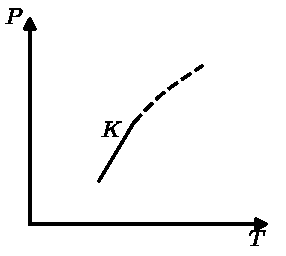
\includegraphics[width=5cm]{fig66.pdf}\\[0.3em]{\small 图 66}\end{minipage}\par\nopagebreak

在展开式(143.3)中，临界点取决于两个系数 $A(P,T)$ 和 $B(P,T)$ 变为零（如果 $A=0$，$B>0$，且有二级相变，则相变曲线只能终止于B变号处）.为使物体的状态在临界点上稳定，五次项必须恒为零，而且六次项为正.因此，我们从如下展开式出发：
\begin{equation}
  \Phi(P,T,\eta)=\Phi_0(P,T)+A(P,T)\eta^2+B(P,T)\eta^4+D(P,T)\eta^6,
\end{equation}
并且在临界点 $A_c=0$，$B_c=0$，$D_c>0$.

在非对称相中，由热力学势取最小，得
\begin{equation}
  \eta^2=\frac{1}{3D}\bigl[-B+\sqrt{B^2-3AD}\bigr].
\end{equation}
忽略 $\eta$ 的高次项，对该相的熵 $S=-\partial\Phi/\partial T$ 有：$S=S_0-a\eta^2$，式中 $a=\partial A/\partial T$.再一次求微商，得热容
\begin{equation}
  C_p=\frac{Ta^2}{2\sqrt{B^2-3AD}},
\end{equation}
此处只写出分母在临界点为零的项.

令温度 $T_0=T_0(P)$ 为满足 $B^2-3AD=0$ 的温度；显然，当 $P=P_c$ 时，$T_0$ 与 $T_c$ 相同.$B^2-3AD$ 按 $T-T_0$ 的幂次展开的第一项为
\begin{equation}
  B^2-3AD=-3a_0D_0(T-T_0).
\end{equation}
在临界点附近，差 $T_c(P)-T_0(P)$ 是二阶小量；事实上，当 $T=T_c(P)$ 时，有 $A=0$，因而差
\begin{equation}
  T_c(P)-T_0(P)=-\frac{B^2}{3a_0D_0},
\end{equation}
也就是说，当 $P\to P_c$ 时，它趋于零如 $B^2$.

把(150.4)代入(150.3)，得
\begin{equation}
  C_p=\Bigl(\frac{T^2a^3}{12D}\Bigr)_c^{1/2}
  \frac{1}{\sqrt{T_0-T}}
\end{equation}
（这个公式中系数取值时可用 $T_c$ 代替 $T_0$ 而仍有同样的精度）.于是，在趋近临界点时，非对称相的热容按 $(T_0-T)^{1/2}$ 增大.

对于正好在二级相变曲线上的状态，令(150.3)中 $A=0$（或者把(150.5)代入(150.6)），得
\begin{equation}
  C_p^{(\mathrm{II})}=\frac{T_ca_c^2}{2B}.
\end{equation}
量B在临界点变为零，在其附近正比于 $T-T_c$（或 $P-P_c$）.

仍然在临界点附近，现在我们确定在一级相变线上非对称相的热容.在这条线的各点上，两种不相同相即对称相和非对称相，彼此平衡.非对称相中参量 $\eta$ 的值取决于平衡条件 $\Phi(\eta)=\Phi_0$，并且同时必须有 $\partial\Phi/\partial\eta=0$.将(150.1)的 $\Phi$ 代入，得方程
\begin{equation*}
  A+B\eta^2+D\eta^4=0,\quad A+2B\eta^2+3D\eta^4=0,
\end{equation*}
因而
\begin{equation}
  \eta^2=-\frac{B}{2D},
\end{equation}
再把这个值代入方程 $\Phi(\eta)=\Phi_0$，给出
\begin{equation}
  4AD=B^2.
\end{equation}
这是一级相变线的方程.

非对称相在这条线上的热容通过将(150.9)代入(150.3)直接得出：
\begin{equation}
  C_p^{(\mathrm{I})}=\frac{T_ca_c^2}{|B|}.
\end{equation}
与(150.7)相比可看出，在离临界点同样远处，一级相变线上的热容是二级相变线上的两倍.从非对称相到对称相的相变热为：
\begin{equation}
  q=T_c(S_0-S)=\Bigl(\frac{aT}{2D}\Bigr)_c|B|.
\end{equation}
还可看出，一级相变曲线在临界点平滑地过渡到二级相变曲线.前一条曲线上，微商 $\mathrm{d}T/\mathrm{d}P$ 取决于条件
\begin{equation*}
  2D\mathrm{d}A+2A\mathrm{d}D-B\mathrm{d}D=0,
\end{equation*}
它由方程(150.9)微分得到.二级相变的曲线方程为 $A=0$，因此 $\mathrm{d}T/\mathrm{d}P$ 取决于条件 $\mathrm{d}A=0$.但是在临界点 $A=0$，$B=0$，所以两个条件一致，$\mathrm{d}T/\mathrm{d}P$ 没有突变.用类似的方式可以证明，二阶微商 $\mathrm{d}^2T/\mathrm{d}^2P$ 经历突变.

沿曲线 $P=P_c$ 趋近临界点时，根据(150.6)热容 $C_p$ 按规律 $|t|^{-1/2}$ 变化，即指数 $\alpha=1/2$.（沿PT平面上所有其它径向趋近时，除了正好在二级相变线即曲线 $A=0$ 的方向上以外，同样的极限规律成立；这时到K点距离起着t的作用.）在非对称相中序参量按规律 $\eta\approx(-A/3D)^{1/4}\propto|t|^{1/4}$ 变化，即指数 $\beta=1/4$.决定关联半径性质的指数 $\nu$，如同在朗道理论中的所有二级相变点处，有同样值 $\nu=1/2$.在推导公式(146.8)的近似下，B变为零并不影响结果.由(148.13)—(148.17)可导得其余指数，值为 $\gamma=1$，$\delta=5$，$\varepsilon=\mu=2/5$，$\zeta=0$.我们已经知道，上述结论所基于的朗道理论在二级相变线附近并不适用.然而，值得注意的是，该理论的适用条件随着临界点的趋近而更易满足，正如不等式(146.15)所示，那里B出现在右边.当然，B变为零并不意味着在临界点完全没有涨落修正.但是，前面所给出的指数值，已经满足标度不变性关系式(149.2).所以很自然，涨落理论的结果与朗道理论结果的区别仅在于到临界点距离的对数项.应该提醒，对数因子不显示在指数值中.

下一步我们考虑（仍在朗道理论框架内）一级和二级相变线交点的某些性质.

在二级相变中非对称相的对称，通过将 $\Phi$ 展开式中的四次项作为系数 $\gamma_i=\eta_i/\eta$ 的函数极小化来决定（正如§145所示）.然而，这些项也与P和T有关，因而有可能出现，在相变线的不同区段非对称相具有各种不同的对称.我们考虑这类情形中最简单的一种：二级相变线（图67的曲线AC）与一级相变线（BD线）相交.区域Ⅰ是对称相；相Ⅱ和Ⅲ的对称群是相Ⅰ对称群的子群.但是，一般说来，它们并非一个为另一个的子群，所以把这两相分开的曲线BD是一级相变线.在B点所有三相等同\footnote{涨落修正也许会导致在B点出现奇异性，线AB和CB形成尖点.}.

\par\nopagebreak\noindent\begin{minipage}{\linewidth}\centering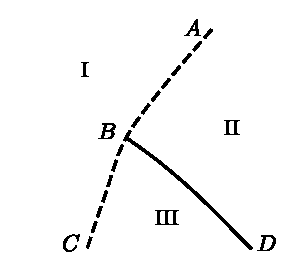
\includegraphics[width=5.5cm]{fig67.pdf}\\[0.3em]{\small 图 67}\end{minipage}\par\nopagebreak

\par\nopagebreak\noindent\begin{minipage}{\linewidth}\centering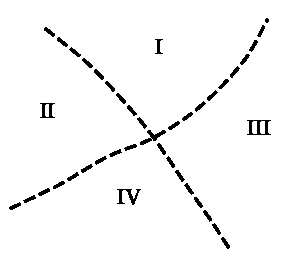
\includegraphics[width=5.5cm]{fig68.pdf}\\[0.3em]{\small 图 68}\end{minipage}\par\nopagebreak

图68图示了几条二级相变线相交的一种可能类型.如果Ⅰ是最对称的相，则相Ⅱ和Ⅲ的对称群是相Ⅰ对称群的子群，而相Ⅳ的对称群是相Ⅱ和Ⅲ的子群\footnote{图67型的交点在文献中称为双临界点，而图68型的交点称为四临界点.如果非对称相之一是无公度相，则双临界点也称为栗弗席兹点（参看本节习题）.——俄文版编者注}.最后，还需要考虑热力学势展开式中三次项不恒为零的情形.在这种情况下，存在连续相变点的条件，要求除系数 $A(P,T)$ 为零外，展开式(145.6)中三次不变式的系数 $C_\alpha(P,T)$ 也该为零.显然，这仅当三次不变式只有一个时才有可能；否则对两个未知量P和T会得到不止两个方程.在只有一个三次不变式时，$A(P,T)=0$ 和 $C(P,T)=0$ 这两个方程决定相应的一对P,T值，即连续相变点是孤立的.

由于这些点是孤立的，它们必定以某种方式位于（在PT平面中）一级相变曲线的交点上.我们不在这里详细研究，只限于指出一些结果\footnote{参看 Ландау Л.~Д. // ЖЭТФ. – 1937. – Т.~7. – С.~19（Собрание трудов. — Т.~1, статья 28. – М.: Наука, 1969.）}.

最简单的类型如图69a所示.相Ⅰ具有的对称较高，而相Ⅱ和Ⅲ较低；这时相Ⅱ和Ⅲ的对称相同，两相区别仅在于 $\eta$ 的符号.在连续相变点（图中的O点），所有三相变为等同.

\par\nopagebreak\noindent\begin{minipage}{\linewidth}\centering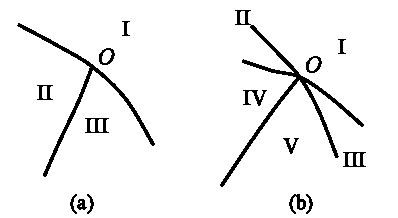
\includegraphics[width=7cm]{fig69.pdf}\\[0.3em]{\small 图 69}\end{minipage}\par\nopagebreak

在更复杂的情况下，有两条（如图69b所示）或更多条一级相变曲线在连续相变点相切.相Ⅰ最对称，其余对称较低，并且相Ⅱ和Ⅲ（以及相Ⅳ和V）的对称相同，而这些相的区别只是 $\eta$ 的符号.

\begin{xiti}

设序参量单分量且只依赖于坐标x，试分析栗弗席兹点附近的相图（A.~Michelson，1977）.

解：栗弗席兹点是可公度相在相变线上的失稳点，对应于在热力学势中 $(\mathrm{d}\eta/\mathrm{d}x)^2$ 项的系数变为零，所以必须考虑 $(\mathrm{d}^2\eta/\mathrm{d}x^2)^2$ 阶次的项：
\begin{equation}
  \Phi_t=\int\Bigl[\Phi_0+A\eta^2+B\eta^4
  +g\Bigl(\frac{\mathrm{d}\eta}{\mathrm{d}x}\Bigr)^2
  +\frac{f}{2}\Bigl(\frac{\mathrm{d}^2\eta}{\mathrm{d}x^2}\Bigr)^2\Bigr]\mathrm{d}V.\tag{1}
\end{equation}
在 $g>0$ 区，具有常数 $\eta$ 的状态即可公度相是稳定的.相应地，
\begin{equation*}
\begin{aligned}
  &g>0,\qquad A>0,\qquad \eta=0\quad(\text{相 I，})\\
  &g>0,\qquad A<0,\qquad \eta=(-A/2B)^{1/2}\quad(\text{相 II}).
\end{aligned}
\end{equation*}
方程 $A(P,T)=0$ 在 $g>0$ 时确定对称相Ⅰ与可公度相Ⅱ之间的二级相变线.栗弗席兹点取决于A和g同时变为零：
\begin{equation*}
  A(P_L,T_L)=0,\qquad g(P_L,T_L)=0.
\end{equation*}
在该点附近，A和g是 $P-P_L$ 和 $T-T_L$ 的线性函数.在 $g<0$ 区相变发生在 $\eta$ 依赖于x的无公度相中.在栗弗席兹点附近，可以认为这种依赖性是纯正弦的：
\begin{equation*}
  \eta(x)=\eta_0\cos qx.
\end{equation*}
将其代入(1)并考虑到 $\overline{\cos^2qx}=1/2$，$\overline{\cos^4qx}=3/8$，可得单位体积的热力学势：
\begin{equation}
  \Phi=\Phi_0+\frac{1}{2}\widetilde{A}(q)\eta_0^2
  +\frac{3}{8}B\eta_0^4,\tag{2}
\end{equation}
式中 $\widetilde{A}(q)=A+gq^2+(f/2)q^4$.如果 $g<0$，当 $q=q_0\equiv(-g/f)^{1/2}$ 时函数 $\widetilde{A}(q)$ 具有极小值.量 $q_0$ 为“调制”波矢.它的波长 $2\pi/q_0$ 以反比于到栗弗席兹点的距离的平方根的方式变成无穷大.最小值 $\widetilde{A}(q_0)=A-g^2/2f$.方程
\begin{equation*}
  \widetilde{A}(q_0)=A-\frac{g^2}{2f}=0
\end{equation*}
决定从对称相Ⅱ到无公度相Ⅲ的二级相变线.将(2)对 $\eta_0$ 求最小，可得调制振幅 $\eta_0^2=(2/3)(-\widetilde{A}/B)$ 和势的值 $\Phi_{\mathrm{III}}=\Phi_0-(1/6)(\widetilde{A}^2/B)$.令 $\Phi_{\mathrm{III}}$ 与公度相的势 $\Phi_{\mathrm{II}}=\Phi_0-(1/4)(A^2/B)$ 相等，可得相Ⅱ和Ⅲ之间的一级相变线的方程
\begin{equation*}
  A=\frac{g^2}{(\sqrt{6}+2)f}.
\end{equation*}
所得的相图大致如图70所示.

\par\nopagebreak\noindent\begin{minipage}{\linewidth}\centering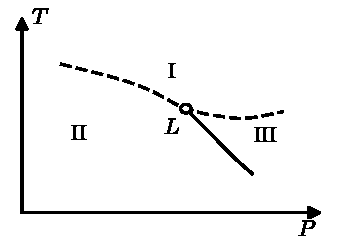
\includegraphics[width=6cm]{fig70.pdf}\\[0.3em]{\small 图 70}\end{minipage}\par\nopagebreak

\end{xiti}

\section{二维晶格中的二级相变}

由于不可能以普遍的形式从理论上定出临界指数，精确解析可解的二级相变问题的简单模型具有特别的意义.有一个特定的二维晶格模型，昂萨格首先解决了其相变问题（L.~Onsager，1944）\footnote{昂萨格原先用的方法极为复杂，以后，许多作者简化了问题的解法.下面所述方法（部分利用了卡茨和沃德方法的某些思想（M.~Kac, J.~C.~Ward, 1952）由 Н.~В.~Вдовиченко（1964）提出.}.

所考虑的模型是由N个格点组成的平面正方晶格，每个格点有一个“偶极子”，其轴垂直于晶格平面.偶极子可以有两个相反的取向，所以偶极子在晶格中的可能组态总数等于 $2^N$\footnote{该模型在文献中以伊辛模型为人所知；实际上它首先由楞次引入（W.~Lenz, 1920），伊辛（E.~Ising, 1925）研究了一维的情形（其中没有相变）.}.我们描述不同的组态如下.每个格点有整数坐标k,l，赋予变量 $\sigma_{kl}$，它可取 $\pm1$ 两个数值，对应于偶极子的两种可能取向.如果仅限于考虑相邻偶极子之间的相互作用，则组态能可以写成
\begin{equation}
  E(\sigma)=-J\sum_{k,l=1}^{L}
  \bigl(\sigma_{kl}\sigma_{k,l+1}+\sigma_{kl}\sigma_{k+1,l}\bigr)
\end{equation}
（L是晶格边的格点数\footnote{当然，假设数L为宏观大，而且以下总是忽略边界效应（与晶格边界附近格点的特殊性有关）.}，晶格设想为大的正方形；$N=L^2$）.参数J决定一对相邻偶极子的相互作用能；对于偶极子的相同和相反的取向，作用能分别等于$-J$和$+J$.以下假设 $J>0$.这时“完全极化的”（有序的）组态具有最小的能量，那里全部偶极子有相同取向.这种组态在绝对零度下实现；随着温度增加，有序程度减小，在相变点变为零，这时候每个偶极子的两种取向变成等概率的.

定义热力学量需要计算配分函数
\begin{equation}
  Z=\sum_{\langle\sigma\rangle}\mathrm{e}^{-E(\sigma)/T}
  =\sum_{\langle\sigma\rangle}\exp\Bigl[\theta\sum_{k,l}
  \bigl(\sigma_{kl}\sigma_{k,l+1}+\sigma_{kl}\sigma_{k+1,l}\bigr)\Bigr],
\end{equation}
此处求和遍及所有可能的 $2^N$ 组态，而 $\theta=J/T$.通过按 $\theta$ 的幂次展开并考虑到所有的 $\sigma_{kl}^2=1$，容易证实，
\begin{equation*}
  \exp\bigl(\theta\sigma_{kl}\sigma_{k'l'}\bigr)
  =\cosh\theta+\sigma_{kl}\sigma_{k'l'}\sinh\theta
  =\cosh\theta\bigl(1+\sigma_{kl}\sigma_{k'l'}\tanh\theta\bigr).
\end{equation*}
所以，表达式(151.2)可以改写成
\begin{equation}
  Z=(1-x^2)^{-N}S,
\end{equation}
式中
\begin{equation}
  S=\sum_{\langle\sigma\rangle}\prod_{k,l=1}^{L}
  \bigl(1+x\sigma_{kl}\sigma_{k,l+1}\bigr)
  \bigl(1+x\sigma_{kl}\sigma_{k+1,l}\bigr)
\end{equation}
而且记 $x=\tanh\theta$.

在(151.4)的求和号后，是变量x和 $\sigma_{kl}$ 的多项式.由于每个格点有四个近邻，每个 $\sigma_{kl}$ 会以零次幂到四次幂出现在多项式中.对所有 $\sigma_{kl}=\pm1$ 的项求和之后，含有 $\sigma_{kl}$ 的奇次幂的项变为零，因此只是含有 $\sigma_{kl}$ 的0,2和4次幂的那些项给出非零的贡献.因为 $\sigma_{kl}^0=\sigma_{kl}^2=\sigma_{kl}^4=1$，所以多项式中含有所有偶次幂的变量 $\sigma_{kl}$ 的每一项，对于和式给出正比于总组态数 $2^N$ 的贡献.

\par\nopagebreak\noindent\begin{minipage}{\linewidth}\centering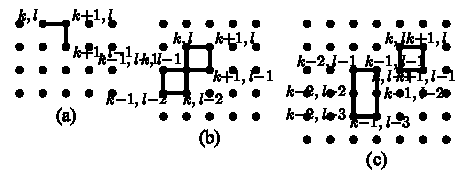
\includegraphics[width=10cm]{fig71.pdf}\\[0.3em]{\small 图 71}\end{minipage}\par\nopagebreak

多项式的每一项可以唯一地对应于一组连接相邻格点对的线或“键”.例如，下列的多项式项与图71所示的图对应：
\begin{equation*}
\begin{aligned}
  &\text{a)}\ \ x^2\sigma_{kl}\sigma_{k+1,l}^2\sigma_{k+1,l-1},\\
  &\text{b)}\ \ x^8\sigma_{kl}^2\sigma_{k+1,l}^2\sigma_{k+1,l-1}^2
  \sigma_{k,l-1}^4\sigma_{k,l-2}^2\sigma_{k-1,l-1}^2\sigma_{k-1,l-2}^2,\\
  &\text{c)}\ \ x^{10}\sigma_{kl}^2\sigma_{k+1,l}^2\sigma_{k+1,l-1}^2
  \sigma_{k,l-1}^2\sigma_{k-2,l-1}^2\sigma_{k-1,l-1}^2\sigma_{k-1,l-2}^2
  \sigma_{k-1,l-3}^3\sigma_{k-2,l-3}^2\sigma_{k-2,l-2}^2.
\end{aligned}
\end{equation*}
图的每一根线赋以因子x，而其每一端点赋以因子 $\sigma_{kl}$.

对配分函数的不为零贡献只来自多项式中含有 $\sigma_{kl}$ 偶次幂的项，这在几何上表示为，应该有两根或者四根键终止在图的每个点.换句话说，求和仅对闭合图进行（这里允许在一点如图71b的点 $(k,l-1)$ 自交）.

于是，和式S可以表示成如下形式
\begin{equation}
  S=2^N{\sum_r}'x^rg_r,
\end{equation}
式中 $g_r$ 是由r（偶数）根键构成的闭合图数；同时每个多连通图（例如，图71c的图）计数为一.

进一步的计算分两步：(1)对上述形式的图形的求和化为对所有可能的闭圈的求和，(2)将所得到的求和化为格点“随机行走”问题计算.

每个图将看成一个或几个闭圈的集合.对于无自交图，这种表示显而易见；比如，图71c是两个圈图的集合.对于自交图，分解方式不唯一；同样的图形可以由数目不同的圈图组成，依赖于构成方法.以图72为例说明，它给出表示图71b的三种方式：一个或两个无自交圈图，或者一个自交圈图.更复杂图的每一自交点可以按这三种方式类似地移动.

\par\nopagebreak\noindent\begin{minipage}{\linewidth}\centering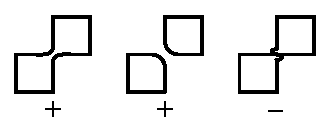
\includegraphics[width=7cm]{fig72.pdf}\\[0.3em]{\small 图 72}\end{minipage}\par\nopagebreak

容易看出，(151.5)的求和可扩充至所有可能的圈图集合，只要在统计图数 $g_r$ 时每图都带上符号 $(-1)^n$，这里n是给定的圈图集合中自交点的总数.实际上，在这样计算时，和式的所有额外项会自动抵消.例如，图72的三图相应地有符号$+$，$+$，$-$，因而其中两个相消，只留下对和式的单个贡献，正该如此.在新的和式中将也含“复键”图，其最简单的例子如图73a所示.这些图属于非容许图（有奇数条即三条键汇于某些点），但是，它们实际上从和式中消失，也正该如此.在构造与这种图对应的圈图时，每条公共键有两种走法：无自交（如图73b）或有自交（图73c），所得的圈图集合在和式中有相反的符号而相消.其次，可以不必直接考虑自交数，如果利用已知的一个几何结果：绕平面闭圈时切线的总旋转角等于 $2\pi(l+1)$，此处l是整数（或正或负），其偶性与圈图自交数 $\nu$ 的偶性一致.所以，如果赋予圈图中的每个格点（旋转角 $\varphi=0,\pm\pi/2$）以因子 $\mathrm{e}^{\mathrm{i}\varphi/2}$，则绕整个圈图后这些因子的乘积给出 $(-1)^{\nu+1}$.对于s个圈图的集合，得因子 $(-1)^{n+s}$，此处 $n=\sum\nu$.

\par\nopagebreak\noindent\begin{minipage}{\linewidth}\centering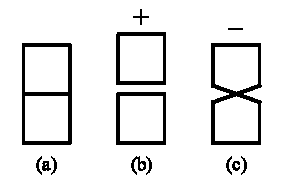
\includegraphics[width=7cm]{fig73.pdf}\\[0.3em]{\small 图 73}\end{minipage}\par\nopagebreak

因此，如果圈图中每个格点加权 $\mathrm{e}^{\mathrm{i}\varphi/2}$ 并对整个图（圈图集合）再引入因子 $(-1)^s$（以抵消 $(-1)^{n+s}$ 中同一因子），则可以不考虑自交数.

用 $f_r$ 记全部长度为r（即由r条键组成）的单圈图之和，并且每个圈图其上各点有因子 $\mathrm{e}^{\mathrm{i}\varphi/2}$.那么，总键数为r的全部二圈图之和等于
\begin{equation*}
  \frac{1}{2!}\sum_{r_1+r_2=r}f_{r_1}f_{r_2}
\end{equation*}
（因子 $\frac{1}{2!}$ 是考虑到指标 $r_1,r_2$ 置换时二圈图不变），对于三圈图等也类似.因此，和式S取如下形式
\begin{equation*}
  S=\sum_{s=0}^{\infty}(-1)^s\frac{1}{s!}
  \sum_{r_1,r_2\cdots=1}^{\infty}x^{r_1+\cdots+r_s}f_{r_1}\cdots f_{r_s}.
\end{equation*}
因为在S中包含具有任意总长度 $r_1+r_2+\cdots$ 的圈图集合，所以在内层求和中，数 $r_1,r_2\cdots$ 可独立地取从1到 $\infty$ 的所有值\footnote{格点数大于N的圈图对求和没有贡献，因为必定含有复键.}.于是，
\begin{equation*}
  \sum_{r_1,\cdots,r_s}x^{r_1+\cdots+r_s}f_{r_1}\cdots f_{r_s}
  =\Bigl(\sum_{r=0}^{\infty}x^rf_r\Bigr)^s,
\end{equation*}
而S化为
\begin{equation}
  S=\exp\Bigl(-\sum_{r=0}^{\infty}x^rf_r\Bigr).
\end{equation}
至此，第一步计算完成.

为了方便后面讨论，指定每一格点有从它出发的四个可能方向，后者用专门指标 $\nu=1,2,3,4$ 编号，比如说按规则
\begin{center}
$\begin{array}{c}
  2\\
  \uparrow\\
  3\leftarrow\ \bullet\ \rightarrow 1\\
  \downarrow\\
  4
\end{array}$
\end{center}
我们引入辅助量 $W_r(k,l,\nu)$，它是从某个给定点 $k_0,l_0,\nu_0$ 到点 $k,l,\nu$ 的长度为r的所有可能路径之和（每键依旧有因子 $\mathrm{e}^{\mathrm{i}\varphi/2}$，此处 $\varphi$ 为走到下一键时方向的改变）；这时走向 $k,l,\nu$ 的最后一步不应该与箭头 $\nu$ 所指的方向相反\footnote{当然，实际上 $W_r(k,l,\nu)$ 仅依赖于差 $k-k_0$，$l-l_0$.}.在这种定义下，$W_r(k_0,l_0,\nu_0)$ 是所有沿 $\nu_0$ 方向从 $k_0,l_0$ 离开而又返回到该点的圈图之和.显然，
\begin{equation}
  f_r=\frac{1}{2r}\sum_{k_0,l_0,\nu_0}W_r(k_0,l_0,\nu_0).
\end{equation}
实际上，上式左右两边均为所有单圈图之和，但是 $\sum W_r$ 包含每个圈图2r次，因为它可以走两个相反方向，而且其r个点的每一个都可取作出发点\footnote{在所叙述的公式(151.8)的推导中有大漏洞；问题在于对和式(151.6)中圈图数所作的计数，并非对任何圈图都正确.例如，一对等同圈图在和式中不出现两次，而是1次.类似地，在(151.7)式中每个圈图出现2r次的结论并非对所有圈图正确.但是，产生的“反常”项在最后的表达式(151.8)中消去了.完全的证明参看 Sherman S. // J. Math. Phys. – 1960. – V.~1 – P.~202; – 1963. – V.~4 – P.~1213. – 俄文版编者注}.把(151.7)代入(151.6)，得
\begin{equation}
  S=\exp\Bigl[-\sum_{r=1}^{\infty}\sum_{k_0,l_0,\nu_0}
  \frac{x^r}{2r}W_r(k_0,l_0,\nu_0)\Bigr].
\end{equation}
从 $W_r(k,l,\nu)$ 的定义有下列递推关系
\begin{equation}
\left.\begin{aligned}
  W_{r+1}(k,l,1)&=W_r(k-1,l,1)+\mathrm{e}^{-\frac{\mathrm{i}\pi}{4}}
  W_r(k,l-1,2)+{}\\
  &\qquad+0+\mathrm{e}^{\frac{\mathrm{i}\pi}{4}}W_r(k,l+1,4),\\
  W_{r+1}(k,l,2)&=\mathrm{e}^{\frac{\mathrm{i}\pi}{4}}W_r(k-1,l,1)
  +W_r(k,l-1,2)+{}\\
  &\qquad+\mathrm{e}^{-\frac{\mathrm{i}\pi}{4}}W_r(k+1,l,3)+0,\\
  W_{r+1}(k,l,3)&=0+\mathrm{e}^{\frac{\mathrm{i}\pi}{4}}W_r(k,l-1,2)+{}\\
  &\qquad+W_r(k+1,l,3)+\mathrm{e}^{-\frac{\mathrm{i}\pi}{4}}W_r(k,l+1,4),\\
  W_{r+1}(k,l,4)&=\mathrm{e}^{-\frac{\mathrm{i}\pi}{4}}W_r(k-1,l,1)+0+{}\\
  &\qquad+\mathrm{e}^{\frac{\mathrm{i}\pi}{4}}W_r(k+1,l,3)
  +W_r(k,l+1,4).
\end{aligned}\right\}
\end{equation}
构成这些关系式的方法是显然的；例如，作最后的第 $r+1$ 步，到达点 $k,l,1$ 时，可从左面，从下面，或者从上面，但是不可从右面；$W_r$ 前的系数来自因子 $\mathrm{e}^{\mathrm{i}\varphi/2}$.

用 $\Lambda$ 表示方程组(151.9)（含所有的k,l）的系数矩阵，可写
\begin{equation*}
  W_{r+1}(k,l,\nu)=\sum_{k',l',\nu'}
  \Lambda(kl\nu\,|\,k'l'\nu')W_r(k',l',\nu').
\end{equation*}
根据构造这个方程组的方法，可赋予这个矩阵一个直观图像：点一步一步地在晶格中“游动”，其每步从一格点到另一个的“转移概率”等于矩阵 $\Lambda$ 的相应元；事实上，仅在k或l只改变0或 $\pm1$ 时矩阵元不为零，即该点每一步只走过一条键.很显然，长度r的“转移概率”将取决于矩阵 $\Lambda^r$.特别是，这个矩阵的对角分量将给出点走完长度为r的一圈后返回出发点的“概率”，即与 $W_r(k_0,l_0,\nu_0)$ 相等.于是，
\begin{equation*}
  \mathrm{tr}\,\Lambda^r=\sum_{k_0,l_0,\nu_0}W_r(k_0,l_0,\nu_0).
\end{equation*}
与(151.7)比较，得
\begin{equation*}
  f_r=\frac{1}{2r}\,\mathrm{tr}\,\Lambda^r
  =\frac{1}{2r}\sum_i\lambda_i^r,
\end{equation*}
式中 $\lambda_i$ 是矩阵 $\Lambda$ 的本征值.把这个表达式代入(151.8)并置换i和r的求和次序，得
\begin{equation}
\begin{aligned}
  S&=\exp\Bigl(-\frac{1}{2}\sum_i\sum_{r=1}^{\infty}\frac{1}{r}x^r\lambda_i^r\Bigr)
  =\exp\Bigl[\frac{1}{2}\sum_i\ln(1-x\lambda_i)\Bigr]={}\\
  &=\prod_i\sqrt{1-x\lambda_i}.
\end{aligned}
\end{equation}
借助于如下傅里叶变换转到其它表示后矩阵 $\Lambda$ 很容易对指标k,l对角化：
\begin{equation*}
  W_r(p,q,\nu)=\sum_{k,l=0}^{L}
  \exp\Bigl[-\frac{2\pi\mathrm{i}}{L}(pk+ql)\Bigr]W_r(k,l,\nu).
\end{equation*}
对方程组(151.9)两边取傅里叶分量后，其中每个方程都只含指标为 $p,q$ 的 $W_r(p,q,\nu)$，即矩阵相对于 $p,q$ 为对角的.对于给定的 $p,q$，其矩阵元等于
\begin{equation*}
  \Lambda(pq\nu\,|\,pq\nu')
  =\begin{pmatrix}
    \varepsilon^{-p} & \alpha^{-1}\varepsilon^{-q} & 0 & \alpha\varepsilon^{q}\\
    \alpha\varepsilon^{-p} & \varepsilon^{-q} & \alpha^{-1}\varepsilon^{p} & 0\\
    0 & \alpha\varepsilon^{-q} & \varepsilon^{p} & \alpha^{-1}\varepsilon^{q}\\
    \alpha^{-1}\varepsilon^{-p} & 0 & \alpha\varepsilon^{p} & \varepsilon^{q}
  \end{pmatrix},
\end{equation*}
式中
\begin{equation*}
  \alpha=\mathrm{e}^{\mathrm{i}\pi/4},\qquad
  \varepsilon=\mathrm{e}^{2\pi\mathrm{i}/L}.
\end{equation*}
对于给定的 $p,q$，简单的计算给出
\begin{equation*}
\begin{aligned}
  \prod_{i=1}^{4}\bigl(1-x\lambda_i\bigr)
  &=\det\bigl(\delta_{\nu\nu'}-x\Lambda_{\nu\nu'}\bigr)={}\\
  &=\bigl(1+x^2\bigr)^2-2x\bigl(1-x^2\bigr)
  \Bigl(\cos\frac{2\pi p}{L}+\cos\frac{2\pi q}{L}\Bigr).
\end{aligned}
\end{equation*}
于是，由(151.3)和(151.10)，最终得配分函数：
\begin{equation}
\begin{aligned}
  Z=2^N\bigl(1-x^2\bigr)^{-N}\times\prod_{p,q=0}^{L}
  \Bigl[\bigl(1+x^2\bigr)^2-{}\\
  -2x\bigl(1-x^2\bigr)
  \Bigl(\cos\frac{2\pi p}{L}+\cos\frac{2\pi q}{L}\Bigr)\Bigr]^{1/2}.
\end{aligned}
\end{equation}
热力学势\footnote{在所考虑的模型中，温度只影响偶极子的取向有序，但不影响其间距（晶格的“热膨胀系数”等于零）.在这种情形下，自由能和热力学势并无实质性差别.}
\begin{equation*}
\begin{aligned}
  \Phi={}&-T\ln Z=-NT\ln 2+NT\ln(1-x^2)-{}\\
  &-\frac{1}{2}T\sum_{p,q=0}^{L}\ln\Bigl[\bigl(1+x^2\bigr)^2
  -2x\bigl(1-x^2\bigr)
  \Bigl(\cos\frac{2\pi p}{L}+\cos\frac{2\pi q}{L}\Bigr)\Bigr]
\end{aligned}
\end{equation*}
或者，将求和变换为积分，得
\begin{equation}
\begin{aligned}
  \Phi={}&-NT\ln 2+NT\ln(1-x^2)-{}\\
  &-\frac{NT}{2(2\pi)^2}\int\!\!\!\int_0^{2\pi}
  \ln\bigl[(1+x^2)^2-2x(1-x^2)(\cos\omega_1+\cos\omega_2)\bigr]
  \,\mathrm{d}\omega_1\mathrm{d}\omega_2,
\end{aligned}
\end{equation}
此处仍记 $x=\tanh(J/T)$.

现在我们考察这个表达式.在被积式对数宗量可变为零的x值处，函数 $\Phi(T)$ 有奇点.作为 $\omega_1$ 和 $\omega_2$ 的函数，这个宗量在 $\cos\omega_1=\cos\omega_2=1$ 时为极小，这时它等于
\begin{equation*}
  \bigl(1+x^2\bigr)^2-4x\bigl(1-x^2\bigr)=\bigl(x^2+2x-1\bigr)^2.
\end{equation*}
这个表达式仅对于x的一个（正）值 $x_c=\sqrt{2}-1$ 有最小值为零；相应的温度 $T_c$（$\tanh\frac{J}{T_c}=x_c$）为相变点.

$\Phi(T)$ 在相变点的附近按 $t=T-T_c$ 幂次的展开，除规则部分外还含有奇异项.在这里我们只对奇异项感兴趣（规则部分直接用它在 $t=0$ 时的值取代）.为求得奇异项的形式，把(151.12)中的对数宗量在其最小值附近按 $\omega_1,\omega_2$ 和t的幂次展开后，该积分取如下形式
\begin{equation*}
  \int\!\!\!\int_0^{2\pi}
  \ln\bigl[c_1t^2+c_2(\omega_1^2+\omega_2^2)\bigr]\,
  \mathrm{d}\omega_1\mathrm{d}\omega_2,
\end{equation*}
式中 $c_1,c_2$ 是常数.积分之后得，在相变点附近热力学势形为
\begin{equation}
  \Phi\approx a+\frac{1}{2}b(T-T_c)^2\ln\left|T-T_c\right|,
\end{equation}
式中a,b仍为常数（且 $b>0$）.热力学势本身在相变点连续，而热容按如下规律变为无穷大：
\begin{equation}
  C\approx-bT_c\ln\left|T-T_c\right|,
\end{equation}
它在相变点的两边是对称的.

在这个模型中，序参量 $\eta$ 由格点平均偶极矩（晶格的自发极化）充当，它在相变点以下不为零，而在以上为零.这个量与温度的依赖关系也可以定下；在相变点附近，序参量按如下规律趋近于零
\begin{equation}
  \eta=\text{常数}\cdot(T_c-T)^{1/8}
\end{equation}
（L.~Onsager，1947）.

关联函数定义为两个格点偶极矩涨落的乘积的平均值.关联半径可证实在 $T\to T_c$ 时按规律 $1/\left|T-T_c\right|$ 趋于无穷大，而在 $T=T_c$ 处，关联函数随距离按如下规律减小
\begin{equation*}
  \left\langle\Delta\sigma_{kl}\Delta\sigma_{mn}\right\rangle
  \propto\bigl[(k-m)^2+(l-n)^2\bigr]^{-1/8}.
\end{equation*}
这些结果，以及解决该模型在外场中性质问题的结果，表明在相变点附近其行为满足标度不变性假设的要求.这时临界指数有下列值：
\begin{equation}
\begin{aligned}
  &\alpha=0,\quad\beta=1/8,\quad\gamma=7/4,\quad\delta=15,\quad\varepsilon=0,\\
  &\mu=8/15,\quad\nu=1,\quad\zeta=1/4
\end{aligned}
\end{equation}
（指数 $\zeta$ 根据(148.7)取 $d=2$ 定）\footnote{值得提醒（参看(148.11)后的脚注），至于临界指数，零指数也对应于对数增长.}.

\section{临界点的范德瓦尔斯理论}

在§83中就已经指出：液气相变的临界点是物质热力学函数的奇点.这种奇异性的物理本质类似于二级相变点奇异性的本质：正如后者与序参量涨落的增大有关，在接近临界点时物质密度的涨落增大.这种在物理本质上的相似性导致这两种现象的可能数学描述有一定的相似性，这将在下节论述.

首先，作为必要的准备，考虑如何基于忽略涨落而描述临界现象.这样的理论（类似于二级相变理论中的朗道近似），假定物质的热力学量（作为变量V和T的函数）没有奇异性，即可以按这些变量的小改变展开为幂级数.因此，本节以下所述的全部结果，只依赖于微商 $(\partial P/\partial V)_T$ 变为零\footnote{热力学量作为变量P，T的函数，这时可有由于变量变换的雅可比式变为零而引起的奇异性.}.

我们先假定
\begin{equation}
  \Bigl(\frac{\partial P}{\partial V}\Bigr)_T=0,
\end{equation}
阐明这时物质的稳定性条件.在§21中推导热力学不等式时，我们从条件(21.1)出发，由之得不等式(21.2)，后者在条件(21.3)、(21.4)下成立.如果(21.4)取等式：
\begin{equation}
  \frac{\partial^2E}{\partial S^2}\frac{\partial^2E}{\partial V^2}
  -\Bigl(\frac{\partial^2E}{\partial V\,\partial S}\Bigr)^2=0,
\end{equation}
则极值条件的这个特殊情形对应于这里感兴趣的情形(152.1).现在二次型(21.2)既可为正，也可为零，视 $\delta S$ 和 $\delta V$ 的值而定；所以量 $E-T_0S+P_0V$ 是否有最小值的问题，需要进一步研究.

显然，我们应该考察的是(21.2)正好取等式的情况：
\begin{equation}
  \frac{\partial^2E}{\partial S^2}(\delta S)^2
  +2\frac{\partial^2E}{\partial S\,\partial V}\delta S\,\delta V
  +\frac{\partial^2E}{\partial V^2}(\delta V)^2=0.
\end{equation}
注意到(152.2)，该等式可以改写成如下形式
\begin{equation*}
  \frac{1}{\partial^2E/\partial S^2}\Bigl(\frac{\partial^2E}{\partial S^2}\delta S
  +\frac{\partial^2E}{\partial S\,\partial V}\delta V\Bigr)^2
  =\frac{1}{\partial^2E/\partial S^2}
  \Bigl[\delta\frac{\partial E}{\partial S}\Bigr]^2
  =\frac{C_v}{T}(\delta T)^2=0.
\end{equation*}
因此，等式(152.3)表明，应该在恒定温度下（$\delta T=0$），考虑对平衡态的偏离.

恒温下，原来的不等式(21.12)变成 $\delta F+P\delta V>0$.把 $\delta F$ 展开成 $\delta V$ 的幂级数并考虑到假设 $\frac{\partial^2F}{\partial V^2}=-(\partial P/\partial V)_T=0$，得
\begin{equation*}
  \frac{1}{3!}\Bigl(\frac{\partial^2P}{\partial V^2}\Bigr)_T\delta V^3
  +\frac{1}{4!}\Bigl(\frac{\partial^3P}{\partial V^3}\Bigr)_T\delta V^4
  +\cdots<0.
\end{equation*}
这个不等式在任意 $\delta V$ 下成立的条件为\footnote{值得指出，(21.3)式取等式的情形，在这里的讨论中不可能，否则条件(21.4)不满足.(21.3)和(21.4)这两个表达式同时变为零也不可能：如果在 $(\partial P/\partial V)_T$ 和 $(\partial^2 P/\partial^2 V)_T$ 变为零的条件上再加一个条件，则两个未知数有三个方程，一般没有公共解.}
\begin{equation}
  \Bigl(\frac{\partial^2P}{\partial V^2}\Bigr)_T=0,\qquad
  \Bigl(\frac{\partial^3P}{\partial V^3}\Bigr)_T<0.
\end{equation}
现在考虑临界点附近的物态方程.这时利用变量T和n代替变量T和V较为方便，这里n是粒子数密度（单位体积内的粒子数）.我们也引入记号
\begin{equation}
  t=T-T_c,\quad p=P-P_c,\quad\eta=n-n_c.
\end{equation}
以这些变量，条件(152.1)和(152.4)可写成
\begin{equation}
  \Bigl(\frac{\partial p}{\partial\eta}\Bigr)_t=0,\quad
  \Bigl(\frac{\partial^2p}{\partial\eta^2}\Bigr)_t=0,\quad
  \Bigl(\frac{\partial^3p}{\partial\eta^3}\Bigr)_t>0,
  \quad\text{当}\ t=0\ \text{时.}
\end{equation}
如果限于按小量t和 $\eta$ 展开的前几项，压强对温度和密度的依赖关系可写成
\begin{equation}
  p=bt+2at\eta+4B\eta^3,
\end{equation}
此处a,b,B为常数.根据(152.6)中的前两个条件，这个展开式没有 $\eta$ 和 $\eta^2$ 的项，而由第三个条件，$B>0$.在 $t>0$ 时，物体的所有均匀态都是稳定的（无处有相分离），即对所有 $\eta$ 应有 $(\partial p/\partial\eta)_t>0$；由此得出，$a>0$.展开式的 $t\eta^2$ 和 $t^2\eta$ 项可略，因为它们必定比 $t\eta$ 项小许多；$t\eta$ 项却应该留下，因为它出现在下面会用到的导数中：
\begin{equation}
  \Bigl(\frac{\partial p}{\partial\eta}\Bigr)_t=2at+12B\eta^2.
\end{equation}
表达式(152.7)决定均匀物质在临界点附近的等温线（图74）.它们的形状和范德瓦尔斯等温线类似（参看图19）.当 $t<0$ 时，它们有最小和最大，而根据条件(84.2)得出的水平段（最下一条等温线的AD）对应于从液态到气态的平衡相变.将条件(84.2)中的V取作分子体积
\begin{equation}
  v=\frac{1}{n}\approx\frac{1}{n_c}-\frac{\eta}{n_c^2},
\end{equation}
该条件可写成
\begin{equation*}
  \int_A^Dv\,\mathrm{d}p=\frac{1}{n_c}(p_2-p_1)
  -\frac{1}{n_c^2}\int_A^D\eta\,\mathrm{d}p=0.
\end{equation*}
但是，平衡中的两相压强相等，$p_1=p_2$，最后得
\begin{equation}
  \int_A^D\eta\,\mathrm{d}p
  =\int_{\eta_1}^{\eta_2}\eta\Bigl(\frac{\partial p}{\partial\eta}\Bigr)_t
  \,\mathrm{d}\eta=0.
\end{equation}
从表达式(152.8)可以看出，被积式是 $\eta$ 的奇函数.所以显然应该有
\begin{equation*}
  \eta_1=-\eta_2.
\end{equation*}

\par\nopagebreak\noindent\begin{minipage}{\linewidth}\centering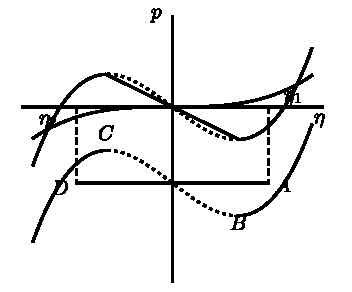
\includegraphics[width=7.5cm]{fig74.pdf}\\[0.3em]{\small 图 74}\end{minipage}\par\nopagebreak

现在运用压强相等条件和公式(152.7)，有
\begin{equation*}
  2at\eta_1+4B\eta_1^3=0.
\end{equation*}
结果得彼此处于平衡的两相密度值如下：
\begin{equation}
  \eta_1=-\eta_2=\sqrt{\frac{-at}{2B}}.
\end{equation}
与亚稳区边界（图74的B点和C点）对应的密度 $\eta_1'$ 和 $\eta_2'$ 取决于条件 $(\partial p/\partial\eta)_t=0$，由此得\footnote{如果将热力学量在亚稳态边界上奇异性考虑在内，则理论通常不包括曲线BC.}.
\begin{equation}
  \eta_1'=-\eta_2'=\sqrt{\frac{-at}{6B}}.
\end{equation}
将(152.11)代入，则(152.7)中最后两项之和为零.于是，
\begin{equation}
  p=bt\qquad(t<0)
\end{equation}
是pt平面中的气液平衡曲线方程（所以 $b>0$）\footnote{当 $t>0$ 时，方程(152.13)决定临界等容线即过临界点的常数密度（$\eta=0$）曲线.}.根据克拉珀龙-克劳修斯方程(82.2)，临界点附近的汽化热为
\begin{equation}
  q\approx bT_c\frac{\eta_1-\eta_2}{n_c^2}.
\end{equation}
因此，从(152.11)可得，当 $t\to0$ 时汽化热按如下规律趋于零
\begin{equation}
  q\propto\sqrt{-t}.
\end{equation}
从公式(16.10)可得，在临界点 $(\partial p/\partial\eta)_t$ 变为零，而同时热容 $C_p$ 变为无穷大.考虑到(152.8)，得
\begin{equation}
  C_p\propto\frac{1}{at+6B\eta^2}.
\end{equation}
特别是，对于平衡曲线上的状态有 $\eta\propto\sqrt{-t}$，所以 $C_p\propto(-t)^{-1}$.

最后，在上述理论框架内考虑临界点附近的密度涨落.必要的普遍公式已在§116中导出，为了运用它们只需要对于物体偏离平衡时总自由能的改变量 $\Delta F_t$ 找出具体形式.

我们把 $\Delta F_t$ 表示成
\begin{equation*}
  \Delta F_t=\int(F-\overline{F})\,\mathrm{d}V,
\end{equation*}
式中F是单位体积的自由能，而 $\overline{F}$ 为其平均值，在物体内为常数.在常数温度下，把 $F-\overline{F}$ 按密度涨落 $\Delta n=n-\overline{n}$（或等价量 $\Delta\eta=\eta-\overline{\eta}$）的幂展开.展开的第一项正比于 $\Delta n$，由于物体中的总粒子数不变，对体积积分后它变为零.二阶项为\footnote{自由能F属于物质的给定（单位）体积，所以 $(\partial F/\partial n)_T=\mu$.二阶导数为 $\bigl(\partial^2 F/\partial n^2\bigr)_T=\bigl(\partial\mu/\partial n\bigr)_T=\frac{1}{n}\bigl(\partial P/\partial n\bigr)_T$（因为在常数T下 $\mathrm{d}\mu=v\,\mathrm{d}P$，此处 $v=1/n$ 是分子体积）.}：
\begin{equation*}
  \frac{1}{2}\Bigl(\frac{\partial^2F}{\partial n^2}\Bigr)_T(\Delta n)^2
  =\frac{1}{2n_c}\Bigl(\frac{\partial P}{\partial\eta}\Bigr)_t(\Delta n)^2.
\end{equation*}
除了在临界点处为零的这一项以外，还应该考虑 $\Delta n$ 的另一二次项，它与密度有涨落的物体的不均匀性有关.在这方面，我们不再重复在§146中给过的讨论，直接指出，该项是 $\Delta n$ 对坐标一阶导数的二次项；在各向同性的介质中，这一项只能是梯度的平方.因此，我们得出如下形式的表达式\footnote{$\Delta F_t$ 表示成了物体中单点函数（而不是一般表达式(116.8)中那样的积分），这与假设 $\Delta n$ 缓变有关，即只考虑密度涨落的长波分量.}
\begin{equation}
  \Delta F_t=\int\Bigl[\frac{1}{2n_c}
  \Bigl(\frac{\partial p}{\partial\eta}\Bigr)_t(\Delta n)^2
  +g\Bigl(\frac{\partial\Delta n}{\partial r}\Bigr)^2\Bigr]\mathrm{d}V.
\end{equation}
现在把 $\Delta n$ 表示为傅里叶级数(116.9)，它可化为(116.10)的形式，其中函数 $\varphi(k)$ 取
\begin{equation*}
  \varphi(k)=\frac{1}{n_c}\Bigl(\frac{\partial p}{\partial\eta}\Bigr)_t+2gk^2
  =\frac{2}{n_c}\bigl(at+6B\overline{\eta}^{\,2}\bigr)+2gk^2,
\end{equation*}
再根据(116.14)，可得待求关联函数的傅里叶变换
\begin{equation}
  \nu(k)=\frac{T}{2}\bigl[at+6B\overline{\eta}^{\,2}+gn_ck^2\bigr]^{-1}
\end{equation}
（由于这个表达式的分母很小，$\nu(k)$ 中的常数1可略）.这个公式完全类似于(146.8).因此，坐标表示的关联函数 $\nu(r)$ 具有(146.11)的同一形式，且关联半径为
\begin{equation}
  r_c=\Bigl(\frac{gn_c}{at+6B\overline{\eta}^{\,2}}\Bigr)^{1/2}.
\end{equation}
特别地，在临界等容线上（$\overline{\eta}=0$）：$r_c\propto t^{-1/2}$.

\section{临界点的涨落理论}

上节所得到的那些公式，使得有可能将临界点类比于二级相变点，对比二者附近物质特性的热力学描述.为此，依照朗道理论的精神，先把 $\eta$ 不当成是P和T的确定函数，而看成独立变量，其平衡值由最小化某个热力学势 $\Phi(P,T,\eta)$ 来确定.后者应该这样选择，以使得这个最小化实际上导致正确的物态方程(152.7).满足这个要求的表达式为\footnote{方括号前的系数在下面并不重要，可以这样选择，使得表达式(153.1)最小化给出正确的势 $\Phi(P,T)$.看似奇怪，在(153.1)中p和t之间不对称，这体现在 $\eta^2$ 前的系数不含p.实际上，仅当 $\eta$ 项的系数 $p-bt$ 很小时 $\eta^2$ 项才重要；在这种情形下，写 $at\eta^2$ 或写 $ap\eta^2/b$ 一样.（另见本节末尾）.}
\begin{equation}
  \Phi(P,T,\eta)=\Phi_0(P,T)
  +\frac{N}{n_c^2}\bigl[-(p-bt)\eta+at\eta^2+B\eta^4\bigr].
\end{equation}
把(153.1)与(144.3)相比较，现在我们看到，在朗道理论对外场中二级相变的描述与范德瓦尔斯理论对气液两相临界点的描述之间存在类似.这时在第二种情形下，物质密度的变化 $\eta=n-n_c$ 相当于序参量，而充当外场的是差
\begin{equation}
  h=p-bt.
\end{equation}
如果 $\Phi(t,h)$ 是物体在二级相变点附近的热力学势（在特定的压强值下），则表达式 $\Phi(t,p-bt)$ 给出了物质在临界点附近热力学势的形式.在§146中有关从势 $\Phi$ 过渡到势 $\Omega$ 的方法的全部论述，适于任意情形，因此在两种问题中的势 $\Omega$ 也有相似性.

在§147中已经指明，如何从朗道理论的热力学势 $\Omega$ 转到有效哈密顿量，用以在精确的涨落理论中描述相变.因此，在上述相似性下可以预料：热力学量在临界点附近行为的规律，等同于外场中（单个序参量描述的）二级相变涨落区的极限规律（适当替换 $\eta$ 和h的意义）.

应该马上强调，这种等同性显然只是一个近似.在基于有效哈密顿量(147.6)的相变理论中，存在关于变换 $h\to-h$，$\eta\to-\eta$ 的精确对称（因三次项$\sim\eta^3$恒为零）.在临界点理论中，这种对称只是近似的；破坏这种对称的项在(153.1)中不存在（因而也不存在于有效哈密顿量中），仅是因为它们与其余项相比很小.所以，只能断定：两种问题的极限关系式中的主导项应该相同\footnote{当然，所描述的相似性不应该掩盖两种现象在物理上的差别：在二级相变的情形下，我们谈论整条的相变点曲线，它在PT平面上分隔不同对称的两相的存在区域，而临界点是孤立点（平衡曲线的终点），位于两相有相同对称的相图中.}.

在相变理论中，在 $t>0$ 且 $h=0$ 时，$\eta=0$；而 $t<0$ 且 $h\to0$ 时，序参量有非零值 $\eta_1$ 和 $\eta_2$ 的两相处于平衡，此处 $\eta_1=-\eta_2$（§144图64b的A和 $A'$ 点）；这里的这个等式是上述的有效哈密顿量对称的精确结果.在临界点的情形下，与这些性质相应的是等式
\begin{equation}
  p-bt=0,
\end{equation}
它决定 $t>0$ 下的等容线（$\eta=0$ 即 $n=n_c$），以及 $t<0$ 下的液汽平衡曲线.在这里，等式 $\eta_2=-\eta_1$ 指示相平衡曲线在 $t\eta$ 平面中的对称性，而扩充的相似性表明这些值在 $t\to0$ 下趋于零，遵从规律
\begin{equation}
  \eta_1=-\eta_2\propto(-t)^{\beta},
\end{equation}
且与(148.5)有同样的指数\footnote{在这里和本节下面，二级相变的临界指数特指用单个序参量描写的且有效哈密顿量形如(147.6)的相变指数值.临界点的范德瓦尔斯理论对应于(148.11)后的脚注中对朗道理论所列出的指数值.}.但是，因为有效哈密顿量（在 $h=0$ 时）对于 $\eta$ 变号的不变性只是近似的，所以产生了关于和式 $\eta_1+\eta_2$ 温度依赖关系的极限规律的问题.根据至今为止的讨论，仅可断定这个量是比 $\eta_1$ 和 $\eta_2$ 本身更高阶的小量；在本节末尾，将再回到这个问题上来.

平面 $\eta t$ 上的相图如图75所示.阴影区表示两相分离区，它的边界为对称曲线，与规律(153.4)一致.

\par\nopagebreak\noindent\begin{minipage}{\linewidth}\centering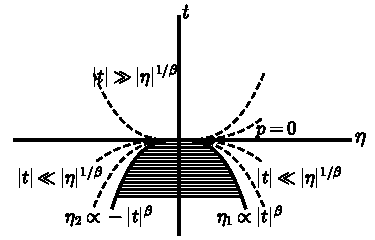
\includegraphics[width=8cm]{fig75.pdf}\\[0.3em]{\small 图 75}\end{minipage}\par\nopagebreak

汽化热与差 $\eta_1-\eta_2$ 有关如公式(152.14)，所以，当 $|t|\to0$ 时它趋于零，遵从同样的规律
\begin{equation}
  q\propto(-t)^{\beta}.
\end{equation}
在临界点的所有邻域内均匀物质的一般物态方程（在平面 $\eta T$ 内）可以表示为
\begin{equation}
  p-bt=\pm\left|\eta\right|^{\delta}
  f\Bigl(\frac{t}{\left|\eta\right|^{1/\beta}}\Bigr),
\end{equation}
式中上、下符号对应于 $\eta>0$ 和 $\eta<0$（B.~Widom，1965）.这个公式对应于相变理论中（在h下解得的）方程(148.18).

在§149已讨论过二级相变中函数 $f(x)$ 的解析性，同样的考虑也适用于(153.6).例如，在给定的非零 $\eta$ 值下，t变号时无处过临界点，因此 $t=0$ 不是函数(153.6)的奇点.于是，它可以按t的整数幂展开.换句话说，函数 $f(x)$ 可按x的整数幂展开.展开的前两项为 $1+c_1x$，结果物态方程取如下形式：
\begin{equation}
  p-bt\propto\pm\left|\eta\right|^{\delta}
  \Bigl(1+c_1\frac{t}{\left|\eta\right|^{1/\beta}}+\cdots\Bigr),
  \quad\text{当}\ \left|t\right|\ll\left|\eta\right|^{1/\beta}\ \text{时；}
\end{equation}
展开式第一项对应于相变理论中强场情况下的定义(148.10).在图75中虚线标示这个状态方程适用区的边界.在该区还可以区分两种极限情况.如果 $t\ll p$（特别是在临界等温线即 $t=0$ 线上），则
\begin{equation}
  p\propto\pm\left|\eta\right|^{\delta}.
\end{equation}
假如 $t\gg p$（特别是在临界等压线即 $p=0$ 线上），则
\begin{equation}
  t\propto\pm\left|\eta\right|^{\delta}.
\end{equation}
把(153.8)和(153.9)相比较可看出，p和t之间存有的对称\footnote{当 $t\propto\eta^{\delta}$ 时，(153.6)中函数 $f(x)$ 的宗量 $x\propto t/t^{1/\beta\delta}\ll1$，因为事实上 $\beta\delta=\beta+\gamma>1$.这证实，在物态方程(153.7)中 $t\gg p$ 的情形实际上是可能的.}.

类似地，对于给定的非零t值，变量 $\eta$ 的零值也不是奇点.所以，在 $t>0$ 且 $\eta\to0$ 时，函数(153.6)可按 $\eta$ 的整数幂展开，而且，同样因为有效哈密顿量对于 $\eta$ 和h的同时变号有对称性，展开式只含 $\eta$ 的奇次幂.由此得出\footnote{$x\to-\infty$ 的情形不现实，因为当 $t<0$ 时，值 $|\eta|^{1/\beta}\ll|t|$ 位于相的分离区.}
\begin{equation*}
  f(x)\propto x^{\beta\delta}
  \bigl(c_1x^{-\beta}+c_3x^{-3\beta}+\cdots\bigr),
  \quad\text{当}\ x\to\infty\ \text{时；}
\end{equation*}
因子 $x^{\beta\delta}$ 约去非整数幂 $\eta^{\delta}$，而展开变量 $x^{-\beta}\propto\eta$.因此，物态方程取如下形式：
\begin{equation}
  p-bt\propto t^{\gamma}\bigl[c_1\eta+c_3\eta^3t^{-2\beta}+\cdots\bigr],
  \quad\text{当}\ t\gg\left|\eta\right|^{1/\beta}\ \text{时，}
\end{equation}
此处已用到等式(148.14)：$\beta\delta=\beta+\gamma$.展开式(153.10)的第一项对应于弱场中相变理论的关系式 $\eta=\chi h\propto ht^{-\gamma}$.

在恒定的t下，p对 $\eta$ 的不同阶导数的行为，依赖于趋近临界点所沿的方向（在 $\eta t$ 平面内）.在沿临界等温线（$t=0$）逼近时，函数 $p(\eta)$ 由公式(153.8)给出.指数 $\delta$ 的实际值在4和5之间.因此，沿临界等温线不仅 $(\partial p/\partial\eta)_t$，而且后几阶导数也趋于零.

在沿任意其它方向（两相分离区之外，即沿射线 $t=$ 常数$\cdot\left|h\right|$，常数$>0$）趋近临界点时，不等式 $t\gg\left|\eta\right|^{1/\beta}$ 成立，因为实际上 $1/\beta>1$.于是，由物态方程有
\begin{equation*}
  \Bigl(\frac{\partial p}{\partial\eta}\Bigr)_t\propto t^{\gamma}\to0,
\end{equation*}
而二阶导数为
\begin{equation*}
  \Bigl(\frac{\partial^2p}{\partial\eta^2}\Bigr)_t
  \propto\eta t^{\gamma-2\beta}=t^{\gamma-\beta}\frac{\eta}{t^{\beta}}.
\end{equation*}
因子 $\eta/t^{\beta}\ll1$，而 $t^{\gamma-\beta}\to0$，因为实际上 $\gamma>\beta$.因此，导数 $(\partial^2p/\partial\eta^2)_t$ 也趋于零.

根据与相变理论中公式(149.7)的相似性，并作指数恒等替换 $\mathrm{d}\nu=2-\alpha$，$\mu/\nu=1/(\beta+\gamma)$，可以直接写出热力学势的表达式
\begin{equation}
  \Phi(p,t)=\left|h\right|^{2-\alpha}
  \varphi\Bigl(\frac{t}{\left|h\right|^{1/(\beta+\gamma)}}\Bigr),
  \quad h=p-bt,
\end{equation}
由之可以推知物质热容在临界区的行为.无须重复所有的讨论，根据同(149.9)和(149.10)的相似性，可立刻写出后面所需要的极限表达式\footnote{值得提醒，这里的 $\Phi$（如同在§149中）指热力学势的奇异部分.它是对非奇异主要部分的小修正，同时它也给出对其它热力学势的同样修正.这里指出，在相平衡曲线上这个附加量的特征值 $\propto t^{2-\alpha}$（这个评注将在§154用到）.}：
\begin{equation}
  \Phi(p,t)\propto t^{2-\alpha}\quad
  \text{当}\ t>0,\ h\to0\ \text{时，}
\end{equation}
\begin{equation}
  \Phi(p,t)\propto(-t)^{2-\alpha}
  \Bigl[1+c_1\frac{\left|h\right|}{(-t)^{\beta+\gamma}}\Bigr]
  \quad\text{当}\ t<0,\ h\to0\ \text{时.}
\end{equation}
对表达式(153.12)两次微商，可得在临界等容线上（$p-bt=0$，$t>0$）的热容
\begin{equation}
  C_v\propto t^{-\alpha}.
\end{equation}
因为在 $h=0$，$t>0$ 下的微商意味着 $\eta=0$ 下的微商，所以有等容热容.因此，临界等容线上的热容 $C_v$ 与二级相变中的热容 $C_p$ 行为相似.

根据公式(16.10)有
\begin{equation*}
  C_p-C_v\propto\frac{(\partial p/\partial t)_\eta^2}{(\partial p/\partial\eta)_t}.
\end{equation*}
在逼近临界点时，导数 $(\partial p/\partial t)_\eta$ 趋于常数极限b，这从物态方程(153.7)或(153.10)容易看出.所以，
\begin{equation}
  C_p\propto\Bigl(\frac{\partial p}{\partial\eta}\Bigr)_t^{-1}.
\end{equation}
趋于临界点时这个表达式发散得比 $C_v$ 快；所以 $C_v$ 项与 $C_p$ 相比后已略去.

最后，我们讨论在临界点附近两相共存曲线的非对称性问题（В.~Л.~Покровский，1972）.正如已经指出的，这种非对称性只可能在以下情况中出现：这时有效哈密顿量含有一些项，破坏了对于变换 $h\to-h$，$\eta\to-\eta$ 的对称.第一个这样的项为$\sim\eta^2h$\footnote{有效哈密顿量添加 $\sim\eta^3 t$ 项，不破坏对称，因为这样的项经施加变换 $\eta\to\eta+$ 常数$\cdot t$ 即可除去.关于这方面可再提一下（参看(149.7)后的脚注），有效哈密顿量中的 $\eta$ 只是连续型积分的变量，因此上述变换并不改变配分函数.}；它的出现在形式上可以认为起因于有效哈密顿量中的t被替换为 $t+$ 常数$\cdot$h；于是
\begin{equation*}
  a\eta^2t\to a\eta^2(t+\text{常数}\cdot h),
\end{equation*}
有效哈密顿量中的这种代换导致在表示成h和t的函数的热力学势中的类似代换：
\begin{equation*}
  \Phi(h,t)\to\Phi(h,t+\text{常数}\cdot h).
\end{equation*}
在两相共存曲线附近，函数 $\Phi(h,t)$ 由表达式(153.13)给出；待求的密度用对h的微分计算.结果得到
\begin{equation*}
  V\eta\big|_{h\to\pm0}=-\Bigl(\frac{\partial\Phi}{\partial h}\Bigr)_{h\to\pm0}
  \propto\mp c_1(-t)^{\beta}
  +(2-\alpha)\cdot\text{常数}\cdot(-t)^{1-\alpha}.
\end{equation*}
第一项给出已知的在对称两相共存曲线上的密度(153.4)；这一项在作求和 $\eta_1+\eta_2$ 后消失，留下
\begin{equation}
  \eta_1+\eta_2\propto(-t)^{1-\alpha},
\end{equation}
它给出所寻求的规律.现实中 $1-\alpha>\beta$\footnote{早已提醒，事实上 $\beta+\gamma>1$.不等式 $1-\alpha>\beta$ 从精确的关系式 $\alpha+2\beta+\gamma=2$ 直接得出.}，非对称性实际上相对较弱：当 $t\to0$ 时，$\frac{\eta_1+\eta_2}{\eta_1}\to0$.和式 $\eta_1+\eta_2$ 实际上为正；这表明，计及非对称项后共存曲线变形如图76所示.

\par\nopagebreak\noindent\begin{minipage}{\linewidth}\centering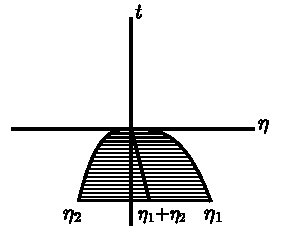
\includegraphics[width=6cm]{fig76.pdf}\\[0.3em]{\small 图 76}\end{minipage}\par\nopagebreak
